\documentclass[11pt]{article}
\usepackage[a4paper,margin=2.4cm]{geometry}
\usepackage[T1]{fontenc}
\usepackage[utf8]{inputenc}
\usepackage{lmodern}
\usepackage{amsmath,amssymb,amsthm,mathtools}
\usepackage{graphicx}
\usepackage{booktabs,tabularx,array}
\usepackage{enumitem}
\usepackage[hidelinks]{hyperref}
\usepackage[capitalise,noabbrev]{cleveref}
\usepackage{xcolor}
\usepackage{microtype}

\setlist{itemsep=2pt,topsep=4pt}
\newenvironment{steps}{\begin{enumerate}[label=\textbf{Step \arabic*.},leftmargin=0pt,itemindent=0pt,labelwidth=!,labelsep=0.5em,align=left,itemsep=7pt,topsep=6pt]}{\end{enumerate}}
\newcommand{\goal}[1]{\par\smallskip\noindent\textit{What we show:} #1\par\smallskip}
\newcommand{\idea}[1]{\noindent\textit{The idea:} #1\par\smallskip}
\setlength{\emergencystretch}{2em}

\newtheorem{theorem}{Theorem}
\newtheorem{lemma}{Lemma}
\newtheorem{proposition}{Proposition}
\newtheorem{corollary}{Corollary}
\theoremstyle{definition}
\newtheorem{definition}{Definition}
\newtheorem{example}{Example}
\theoremstyle{remark}
\newtheorem{remark}{Remark}

\newcommand{\R}{\mathbb{R}}
\newcommand{\Ustar}{\mathcal{U}^{*}}
\newcommand{\GCM}{\operatorname{GCM}}
\newcommand{\LCM}{\operatorname{LCM}}
\newcommand{\qbar}{\bar q}
\newcommand{\cC}{\mathcal{C}}
\newcommand{\cU}{\mathcal{U}}
\newcommand{\tier}[1]{\textsc{#1}}
\newcommand{\authorinput}[1]{\textcolor{red}{[AUTHOR INPUT NEEDED: #1]}}

\title{Flat shoulders break the uniform calibration of the dip test,\\
and a constant cutoff repairs it}
\author{\textbf{Moemen Ahmed}\\[4pt]
\normalsize Independent Researcher\\[4pt]
\small momen.ashraf.3101@gmail.com\quad$\cdot$\quad ORCID 0009-0002-3464-7067\\[3pt]
\small Code and data: {\urlstyle{same}\url{https://github.com/MomenAhmed05/dip-test-calibration}}}
\date{}

\begin{document}
\maketitle

\begin{abstract}
The dip test of Hartigan and Hartigan (1985) is the standard nonparametric test of unimodality. It measures how far the empirical distribution function of a sample lies from the nearest unimodal distribution function, that is, from a distribution function that curves upward (is convex) until the peak of the density and curves downward (is concave) after it. Its critical values are taken from the uniform distribution, on the grounds that among unimodal laws the uniform produces the largest dip. We show that this is false. Consider a density that is flat over most of its range and then jumps up to a narrow peak at one end. Because the peak sits at the end of the flat stretch, every good unimodal fit to the sample must keep curving upward over the whole flat stretch, and it can no longer bend to follow random bumps in the data. In large samples the dip then behaves like half the largest gap between a Brownian bridge and its concave majorant, a quantity whose law was found by Balabdaoui and Pitman (2011), and this quantity is stochastically larger than the uniform limit of the dip. With 90 percent of the mass on the flat stretch, the nominal 5 percent test rejects about one sample in four, however large the sample.

We prove that over atomless unimodal laws with bounded support and a finite density at the mode, the worst limiting rejection rate of the standard 5 percent test lies between 28.4 and 33.2 percent, and between 12.7 and 16.8 percent at the 1 percent level; the width of these intervals comes from a certified numerical bracket for the limiting uniform critical value. Rejecting when the dip exceeds $c_\alpha/\sqrt n$, where $c_\alpha$ is half the $(1-\alpha)$ quantile of the Balabdaoui--Pitman gap ($c_{0.05}\approx0.7314$ and $c_{0.01}\approx0.8599$), restores the nominal level on that class in the limit, and no deterministic sequence of cutoffs with a smaller limit does. A computer-assisted argument, based on Monte Carlo certificates with a stated error probability, shows that the same intervals hold when the worst law is chosen separately at each sample size among all continuous unimodal laws. We also give certified cutoffs for small and moderate samples, and we measure the price of the correction: on symmetric normal mixtures the corrected test needs about twice as many observations as the uniform-calibrated one to reach the same power.
\end{abstract}

\section{Introduction}\label{sec:intro}

\subsection{Motivation}
Suppose an analyst has a few hundred measurements and wants to know whether they come from one population or from a mixture of two. A histogram with two humps suggests two groups, but histograms show humps by chance, so the analyst wants a test. The usual choice is the dip test of Hartigan and Hartigan \cite{HH85}. It measures how far the empirical distribution function is from the nearest unimodal distribution function, and it rejects unimodality when that distance, the dip, is large. It needs no bandwidth and no parametric model, it is available in the R package \texttt{diptest} \cite{Maechler}, and clustering methods call it to decide whether a group should be split \cite{Maurus16,Bauer23}.

Whether the dip is ``large'' depends on what a unimodal law usually produces, and that depends on which unimodal law generated the data. Hartigan and Hartigan dealt with this by calibrating at one law. They took critical values from the uniform distribution and stated, in their abstract, that the uniform is asymptotically the least favourable unimodal distribution: among unimodal laws, it is supposed to produce the largest dips. If that holds, the uniform critical values are safe for every unimodal null, and conservative for most. Cheng and Hall \cite{CH98} later quantified the conservative side: for smooth laws with a well-defined peak, the rejection rate of the uniform-calibrated test tends to zero as the sample grows. Practitioners have reasonable grounds, then, to treat the uniform calibration as cautious.

\subsection{A unimodal law that the standard test rejects too often}
It is not cautious for every unimodal law. Consider the two-step density that spreads 90 percent of the mass evenly over $(0,0.995)$ and puts the remaining 10 percent on the narrow interval $(0.995,1)$. This law is unimodal: its density rises once, at $0.995$, and never falls back. \Cref{fig:fixedlaw} shows how often the standard 5 percent dip test rejects samples from it. At $n=200$ the rate is already 26 percent, and it stays near 25 percent up to $n=12{,}800$, the largest size we simulated. At the 1 percent level the rate settles near 10 percent. The same samples tested with the cutoff we propose are rejected at most about 3 percent of the time at the 5 percent level and 0.5 percent of the time at the 1 percent level.

\begin{figure}[t]
\centering
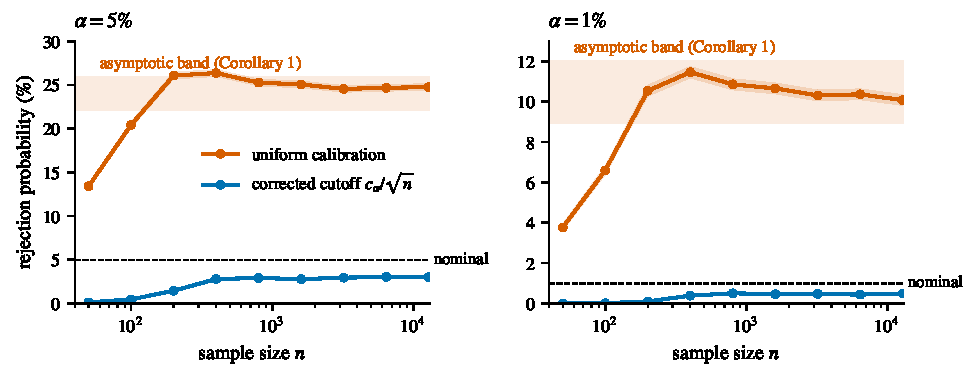
\includegraphics[width=\linewidth]{figs/fig3_fixed_law.pdf}
\caption{For this unimodal law the standard dip test rejects about a quarter of the samples at the nominal 5 percent level, and the excess does not shrink as $n$ grows. Rejection rates for the law with 90 percent of the mass spread evenly on $(0,0.995)$ and 10 percent on $(0.995,1)$, as the sample size grows. Orange: the standard dip test with uniform critical values. Blue: the constant cutoff $c_\alpha/\sqrt n$ proposed in \cref{sec:size}. Each point uses $50{,}000$ samples; the shaded strips around the lines are 95 percent intervals. The orange band is the asymptotic lower bound of \cref{cor:shoulder}, evaluated over the certified range of the limiting uniform critical value. The rejection rate of the standard test does not fall back towards the nominal level as $n$ grows.}
\label{fig:fixedlaw}
\end{figure}

Hartigan and Hartigan knew that the uniform is not least favourable at $n=4$; their paper gives a counterexample at that sample size \cite[p.~73]{HH85}. Müller \cite{Mueller92} suspected that certain bi-uniform laws are worse than the uniform, and Mächler's vignette for \texttt{diptest} calls the uniform ``not quite'' least favourable. None of these works shows a failure in large samples or measures how large it can be. \Cref{fig:fixedlaw} is a failure in large samples, and the rest of this paper explains it and gives a cutoff that removes it.

\subsection{The mechanism in brief}
It helps to keep two pictures side by side. A unimodal density rises to a peak and then falls. Its distribution function, which is what the dip test works with, therefore rises with increasing slope up to the peak, so it curves upward (is convex) there, and rises with decreasing slope after the peak, so it curves downward (is concave). We call the point where the curvature changes from upward to downward the \emph{turning point} of the distribution function; it sits at the mode of the density. To compute the dip, one looks for the unimodal distribution function closest to the empirical one, and that fit may put its turning point anywhere. Under the uniform law the fit uses this freedom: it bends wherever the random fluctuations of the sample make bending cheapest. The two-step law takes the freedom away. Its density jumps up at $0.995$, so the distribution function becomes much steeper there, and any fit that stays close to it must still be steepening at $0.995$. A unimodal fit stops steepening at its turning point, so the turning point of every close fit has to lie in the narrow top, and over the whole long flat part the fit has to curve upward. The random fluctuations of the empirical distribution function on that flat part look, at scale $n^{-1/2}$, like a Brownian bridge, and the best upward-curving (convex) fit to a Brownian bridge misses it by half the largest gap between the bridge and its greatest convex minorant. That half-gap is stochastically larger than the uniform limit of the dip, and this is why the test rejects too often. \Cref{sec:mechanism} turns this paragraph into a theorem.

\subsection{Contributions}
\begin{enumerate}[label=(\arabic*),leftmargin=*]
\item \emph{The failure.} For every level $\alpha\in(0,1)$ there is a fixed two-step unimodal law whose rejection probability under the uniform calibration stays above $\alpha$ by a fixed margin for all large $n$. The proof uses no numerical input (\cref{sec:mechanism}).
\item \emph{Its size.} Over atomless unimodal laws on a bounded interval with finite density at the mode, no law has a limiting rejection rate above $1-F_M(2\qbar_\alpha)$ under the standard test, and some laws come arbitrarily close to it. Here $F_M$ is the distribution function of the Balabdaoui--Pitman gap and $\qbar_\alpha$ is the limiting uniform critical value. Numerically this is 28.4 to 33.2 percent at the 5 percent level and 12.7 to 16.8 percent at 1 percent (\cref{sec:size}).
\item \emph{The correction.} The cutoff $c_\alpha/\sqrt n$, with $c_\alpha=\tfrac12F_M^{-1}(1-\alpha)$, keeps the limiting rejection rate at or below $\alpha$ for every law in that class, and no deterministic sequence of cutoffs with a smaller limit does (\cref{sec:size}).
\item \emph{The worst case at a given sample size.} We show that for every $n$, the rejection probability under any continuous unimodal law is at most that of a uniform sample whose fit is forced to turn at a fixed point. With this reduction and a computer-assisted argument we place the large-sample limit of the worst-case size in the same intervals as in (2) (\cref{sec:worst}).
\item \emph{Finite samples.} Certified cutoffs at $n=4$, at every $n$ from 8 to 49, and at six values of $n$ from 50 to 1600, together with enclosures of the size of the standard test at 21 sample sizes from 4 to 1000 (\cref{sec:finite}).
\item \emph{The cost.} The corrected test needs about twice the sample size of the uniform-calibrated test for the same power on symmetric normal mixtures, and in simulated clustering pipelines it removes most spurious splits of unimodal features that have flat parts (\cref{sec:practice}).
\end{enumerate}

\subsection{Scope and how the results were checked}
All results assume independent, identically distributed observations from a continuous distribution. Items (1) to (3) are theorems with written proofs. Item (4) combines proved reductions with a Monte Carlo certificate: a computation whose decision rule was fixed in advance and whose probability of certifying a false statement is bounded, by 0.01 or less in this paper. Items (2) to (4) also use the convergence of the scaled uniform critical values to $\qbar_\alpha$, which holds if the distribution function of the limiting uniform dip has neither a jump nor a flat stretch at $\qbar_\alpha$; we assume this, and simulation supports it (\cref{sec:setting}). The numerical constants are either enclosed rigorously by interval arithmetic or certified in the same Monte Carlo sense; \cref{sec:numbers} explains the difference. The deterministic steps of several arguments were also checked in the Lean proof assistant \cite{Lean4} with the Mathlib library \cite{Mathlib}. The code, the deposited outputs and the Lean files are in the repository named under the title.

\section{The dip test and two limit laws}\label{sec:setting}

This section sets up the objects the rest of the paper compares: the dip, the uniform critical values, the limit law that the uniform calibration is built on, and the limit law that replaces it on a flat shoulder.

\subsection{The dip}
A distribution function $F$ is \emph{unimodal} if, for some point $m$, it is convex to the left of $m$ and concave to the right. Equivalently, its density rises up to $m$ and falls after it. Flat stretches are allowed, and so is a modal interval instead of a single mode. This is the definition of Hartigan and Hartigan \cite{HH85}, and we use it throughout. We call $F$ \emph{continuous unimodal} if in addition it has no atom.

The dip of a distribution function $G$ is its largest vertical distance to the nearest unimodal distribution function. For a sample $X_1,\dots,X_n$ with empirical distribution function $F_n$, the dip statistic is $D_n=D(F_n)$. The dip does not change under an increasing affine change of variable, so we may put the data in $[0,1]$. Hartigan and Hartigan \cite[Theorem~1]{HH85} also showed that the constraint ``is a distribution function'' can be dropped: for $G$ on $[0,1]$, $D(G)$ equals the distance from $G$ to the bounded functions that are convex on $[0,m]$ and concave on $[m,1]$ for some $m$. We call $m$ the \emph{turning point} of such a function. This form lets us take the dip of any bounded function $h$, which we need because the limits below are dips of random continuous functions.

The argument uses a one-sided version of the dip, the distance to the nearest convex function. The \emph{convex distance} of a bounded function $h$ on an interval $I$ is
\[
V_I(h)=\inf\Bigl\{\sup_{x\in I}|h(x)-g(x)| : g \text{ convex on } I\Bigr\},
\]
and we write $V(h)$ when $I=[0,1]$. The \emph{concave distance} $C_I(h)$ is defined in the same way with concave functions in place of convex ones. A convex function is a unimodal fit whose turning point sits at the right end, so $D(h)\le V(h)$ always. The dip can choose its turning point and the convex distance cannot. \Cref{sec:mechanism} shows that a flat shoulder takes this choice away.

\subsection{The uniform calibration}
Under the uniform law on $[0,1]$ the distribution of $D_n$ depends only on $n$. Let $q_n(1-\alpha)$ be its $(1-\alpha)$ quantile. The \emph{standard test} at level $\alpha$ rejects unimodality when $D_n\ge q_n(1-\alpha)$. We always mean the exact uniform quantile here, so simulation error in published tables plays no role.

Hartigan and Hartigan proved that under the uniform law $\sqrt nD_n$ converges in distribution to $D(B)$, the dip of a standard Brownian bridge $B$ \cite[Theorem~3]{HH85}. Let $\qbar_\alpha$ be the $(1-\alpha)$ quantile of $D(B)$. If the distribution function of $D(B)$ has neither a jump nor a flat stretch at $\qbar_\alpha$, the scaled critical values converge, $\sqrt n\,q_n(1-\alpha)\to\qbar_\alpha$. This condition is not proved, but every simulation we ran supports it, and we assume it wherever a result is stated in terms of $\qbar_\alpha$. Roughly, $\qbar_{0.05}\approx0.546$ and $\qbar_{0.01}\approx0.63$; certified ranges follow in \cref{sec:numbers}.

\subsection{The concave-majorant gap}
The second limit law comes from a different functional of the bridge. Let $\LCM(B)$ be the least concave majorant of $B$ on $[0,1]$, the smallest concave function lying above it, and let
\[
M=\sup_{0\le u\le1}\bigl(\LCM(B)(u)-B(u)\bigr)
\]
be the largest vertical gap between the two. Balabdaoui and Pitman \cite{BP11} found the law of $M$; it has a density and mean about $0.9994$. Balabdaoui and Filali \cite{BF11} tabulated its distribution function, which we write $F_M$. Since $-B$ is again a Brownian bridge, the largest gap between $B$ and its greatest convex minorant also has the law of $M$; this is the form in which $M$ appears in \cref{sec:mechanism}. We define
\[
c_\alpha=\tfrac12F_M^{-1}(1-\alpha),
\]
so that $P(M/2>c_\alpha)=\alpha$. Its values are $c_{0.10}\approx0.668$, $c_{0.05}\approx0.7314$ and $c_{0.01}\approx0.8599$. \Cref{fig:limits} compares the two limit laws. At the uniform 5 percent cutoff $\qbar_{0.05}$, the law of $M/2$ still has about 30 percent of its mass to the right.

\begin{figure}[t]
\centering
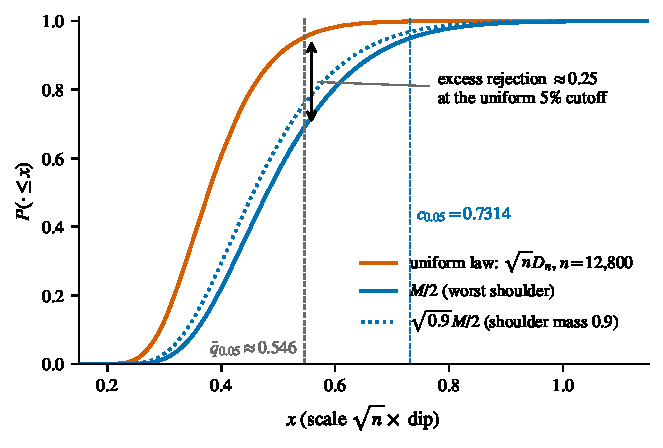
\includegraphics[width=0.78\linewidth]{figs/fig2_limit_laws.pdf}
\caption{At the uniform 5 percent cutoff, the shoulder limit $M/2$ still puts about 30 percent of its mass above the cutoff, while the uniform limit puts 5 percent there. Orange: the distribution function of $\sqrt nD_n$ under the uniform law, from $10^5$ simulated samples at $n=12{,}800$; its 95 percent point is close to $\qbar_{0.05}\approx0.546$. Solid blue: the distribution function of $M/2$, from the table of Balabdaoui and Filali. Dotted blue: $\sqrt{0.9}\,M/2$, the shoulder term for a shoulder of mass 0.9; for the running example the full limit is the larger of this term and an independent term $\sqrt{0.1}\,D(B')$ from the top, which hardly ever matters at these cutoffs (\cref{sec:mechanism}). The vertical distance between the curves at $\qbar_{0.05}$ is the excess rejection rate that a shoulder of nearly full mass produces. The constant $c_{0.05}=0.7314$ is the 95 percent point of $M/2$.}
\label{fig:limits}
\end{figure}

\subsection{Limiting rates and worst cases}
Rejection probabilities need not converge, and we never need them to. When we say that a limiting rejection rate is at most $x$, we mean that its limit superior is at most $x$; when we say it is at least $x$, we mean its limit inferior.

Two questions about the null hypothesis sound alike but are different. The first fixes a law $F$, lets $n$ grow, and then asks for the worst law; this is the \emph{pointwise} question, answered in \cref{sec:mechanism,sec:size}. The second fixes $n$, takes the worst law at that $n$,
\[
S_n(\alpha)=\sup_{F\ \text{continuous unimodal}}P_F\bigl(D_n\ge q_n(1-\alpha)\bigr),
\]
and then lets $n$ grow; this is the \emph{worst-case size} $S_n(\alpha)$, the quantity a user who does not know the law actually faces. It is at least as large as the pointwise answer, because a law that changes with $n$ is allowed. \Cref{sec:worst} shows that, for the dip, both answers lie in the same interval.

For the pointwise results we need a class of laws regular enough to analyse. Let $\cC$ be the atomless unimodal laws on a bounded interval whose one-sided densities at the mode are finite. It contains every unimodal step density, trapezoids, the triangular law, Beta$(a,b)$ laws with $a,b>1$ and truncated normal laws. It excludes unbounded support, an infinite density at the mode and atoms.

\subsection{What the numbers guarantee}\label{sec:numbers}
Several constants in this paper are computed, and we use two kinds of guarantee for them.

A value is \emph{rigorously enclosed} when it is computed in ball arithmetic, which carries every rounding error into the result. We enclose $F_M$ on a fine grid with the Arb library \cite{Arb}, starting from the stick-breaking representation of Balabdaoui and Pitman with an explicit bound on the remainder of its series. This gives $c_{0.10}\in[0.667,0.6685]$, $c_{0.05}\in[0.7305,0.7325]$ and $c_{0.01}\in[0.8585,0.861]$. A finer floating-point enclosure, which pads the error but is not rigorous in the same sense, gives $c_{0.05}\in[0.7313,0.7315]$ and $c_{0.01}\in[0.8598,0.8599]$.

A value is \emph{certified} when it comes from a Monte Carlo computation whose code, random seeds, sample size and decision rule were fixed in a written protocol before it ran, and whose decision rule uses exact binomial or Bernstein bounds with a correction for every claim in the run. If the claimed statement were false, the run would certify it with probability at most a stated $\delta$. The probability refers to the random draws, not to the statement. In this way we bracket the limiting uniform critical values: from $12{,}000$ simulated bridges on a grid of $2\cdot10^6$ points, with lower and upper bounds on $D(B)$ for each path,
\[
\qbar_{0.05}\in[0.5379,\,0.5558],\qquad \qbar_{0.01}\in[0.6162,\,0.6438],
\]
jointly with confidence at least $0.99$, and $\qbar_{0.10}\in[0.4936,\,0.5108]$ with confidence at least $0.998$. The value $0.5452$ in the \texttt{diptest} table at $n=72{,}000$ lies inside the first bracket. Most of the width of the size intervals quoted later comes from these brackets.

\subsection{Related work}\label{sec:prior}
Besides the work cited in \cref{sec:intro}, three lines of research are close to ours. Müller and Sawitzki \cite{MS91} and Polonik \cite{Polonik95} developed the excess-mass approach to modality; in one dimension the excess-mass statistic for two modes equals twice the dip \cite{CH98}. Cheng and Hall \cite{CH98} replaced the uniform calibration by one fitted to the curvature at the mode, and in a second paper \cite{CH99} showed that a shoulder near the mode makes such calibrations anticonservative and proposed a shoulder-aware version. Their shoulders are smooth; ours are stretches of constant density that end in a jump. Davies and Kovac \cite{DK04} used a Kuiper-type distance, which gives a conservative cutoff for the dip that is valid at every $n$, and Hartigan \cite{Hartigan00} proposed a statistic aimed at shoulders and antimodes.

For the one-sided question, whether a distribution function is concave, the uniform \emph{is} least favourable. Kulikov and Lopuhaä \cite{KL08} proved this for the supremum distance to the least concave majorant, even at fixed $n$, Carolan \cite{Carolan02} obtained closely related results, and Beare \cite{Beare21} extended least favourability to $L^p$ distances in the limit. Carolan and Dykstra \cite{CD99} studied the Grenander estimator at flat regions of a density, a one-sided version of the effect that flat stretches have here. Beare and Fang \cite{BF17} computed the directional derivative of the least concave majorant at a distribution function with affine pieces, a tool we use. The one-sided results do not carry over to the dip because the dip lets its fit turn, and the turning point is exactly what a flat shoulder constrains.

\section{Flat shoulders and the convex fit}\label{sec:mechanism}

This section proves that the uniform calibration fails, and shows where the law of $M$ enters. The argument has three ingredients: an exact formula for the convex distance, a condition that forces the fit to be convex on a stretch of the data, and the Brownian limit of the empirical process on that stretch.

\subsection{The picture}
Write $W(w,\varepsilon)$ for the two-step law on $[0,1]$ whose density equals $(1-w)/(1-\varepsilon)$ on $(0,1-\varepsilon)$ and $w/\varepsilon$ on $(1-\varepsilon,1)$, with $0<\varepsilon<w<1$. The long flat part carries mass $1-w$; we call it the \emph{shoulder}. The short interval at the right end carries mass $w$ and has a much higher density; we call it the \emph{top}. The law in \cref{fig:fixedlaw} is $W(0.1,0.005)$, and we use it as a running example. \Cref{fig:mechanism}(a) shows the shape.

\begin{figure}[t]
\centering
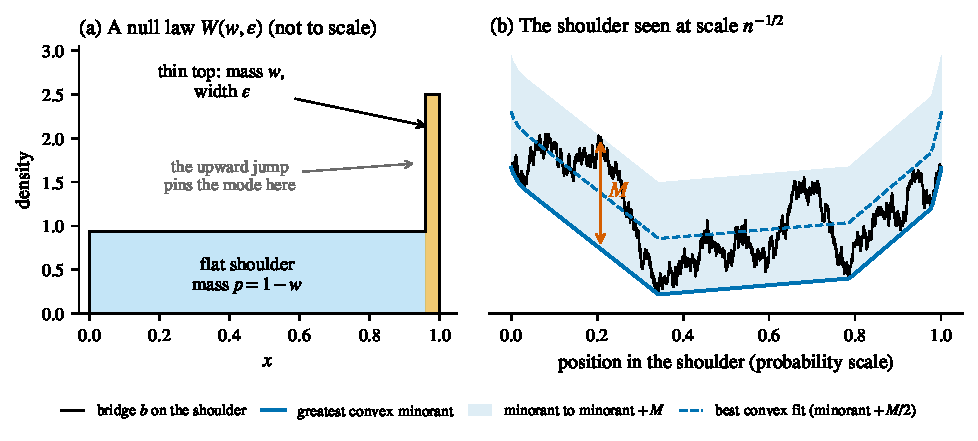
\includegraphics[width=\linewidth]{figs/fig1_mechanism.pdf}
\caption{A pinned shoulder forces the fit to curve upward over the whole shoulder, and the best such fit to a Brownian bridge misses it by half the largest gap $M$. (a) The null law $W(w,\varepsilon)$: a flat shoulder of mass $1-w$ followed by a thin top. Because the density jumps up at the start of the top, every close unimodal fit must turn to the right of any fixed point inside the shoulder, so the fit is convex there. (b) After removing its chord and rescaling, $\sqrt n(F_n-F)$ on the shoulder is close in law to $\sqrt{1-w}$ times a Brownian bridge; one simulated bridge $b$ is shown. A convex function within distance $d$ of $b$ lies below the greatest convex minorant plus $d$, so it cannot reach the top of the largest gap $M$ unless $d\ge M/2$. The minorant shifted up by $M/2$ (dashed) attains this. Under the uniform law the fit may turn anywhere, which gives the smaller limit $D(B)$.}
\label{fig:mechanism}
\end{figure}

Imagine fitting a unimodal distribution function to a large sample from $W(0.1,0.005)$. The true distribution function rises slowly along the shoulder and then very steeply over the top. A good fit must follow that steep rise, so it must still be rising steeply at $0.995$; a unimodal distribution function rises fastest at its mode, so the fit's turning point has to sit in the top. Over the whole shoulder, then, the fit is on the convex side of its turning point. It cannot bend the other way to follow a random bump in the data, as it could under the uniform law. On the shoulder the dip is therefore at least the convex distance of the data, and the next two results evaluate that distance.

\subsection{The half-gap identity}
The first result is an identity. It says that the best convex fit to any function is its greatest convex minorant lifted by half the largest gap.

\begin{lemma}[half-gap identity]\label{lem:halfgap}
For a bounded function $h$ on a compact interval $I$,
\[
V_I(h)=\tfrac12\sup_{x\in I}\bigl(h(x)-\GCM_I(h)(x)\bigr),
\]
where $\GCM_I(h)$ is the greatest convex minorant of $h$ on $I$. In particular $V(B)$ has the law of $M/2$.
\end{lemma}
\begin{proof}
Let $G$ be the largest gap on the right. The function $\GCM_I(h)+G/2$ is convex and lies within $G/2$ of $h$, so $V_I(h)\le G/2$. For the reverse inequality take any convex $g$ with $\sup_I|h-g|\le d$. Then $g-d$ is a convex function below $h$, so it lies below the greatest convex minorant, and at every $x$, $h(x)-\GCM_I(h)(x)\le h(x)-g(x)+d\le2d$. Hence $G\le2d$. The law of $V(B)$ follows because $-B$ is again a Brownian bridge.
\end{proof}

Panel (b) of \cref{fig:mechanism} is this proof drawn for one simulated bridge. On a piece of a bridge the same identity applies after rescaling: the bridge restricted to an interval of length $s$, with its chord removed, is $\sqrt s$ times a standard bridge independent of the rest (\cref{lem:pieces} in \cref{app:proofs}), so its convex distance has the law of $\sqrt s\,M/2$.

\subsection{Pinned shoulders}
Two properties of $W(w,\varepsilon)$ drive the argument above, and we isolate them.

\begin{definition}[pinned shoulder]\label{def:shoulder}
A unimodal distribution function $F$ on $[0,1]$ has a \emph{pinned shoulder of mass $p$} if, for some $0<L<1$,
\begin{enumerate}[label=(\roman*),leftmargin=*]
\item $F$ is linear on $[0,L]$ with $F(L)=p$; and
\item for every $\delta\in(0,L)$ the concave distance $\kappa_\delta=C_{[L-\delta,1]}(F)$ is positive.
\end{enumerate}
\end{definition}
Condition (i) is the flat shoulder. Condition (ii) is the pin: a unimodal fit that turned inside the shoulder would have to be concave on some interval $[L-\delta,1]$, and (ii) says that $F$ stays at least $\kappa_\delta$ away from every such function. For $W(w,\varepsilon)$ the pin is the upward jump of the density at $L=1-\varepsilon$, and $p=1-w$. The $n=4$ counterexample of Hartigan and Hartigan, a uniform law with an atom at its right end, has a pinned shoulder too, with the atom in place of the top.

\begin{theorem}[pinned shoulders]\label{thm:shoulder}
If $F$ has a pinned shoulder of mass $p$, then for every $t\ge0$
\[
\liminf_{n\to\infty}P_F\bigl(\sqrt nD_n>t\bigr)\ \ge\ P\bigl(\sqrt p\,M/2>t\bigr).
\]
\end{theorem}

The proof in \cref{app:proofs} follows the picture. First, with probability tending to one the sample is close enough to $F$ that the pin rules out every fit turning inside $[0,L-\delta]$, so the dip is at least the convex distance of $F_n$ on that interval. Second, $F$ is linear there, and adding a linear function does not change a convex distance, so the convex distance of $F_n$ equals that of $F_n-F$; by Donsker's theorem $\sqrt n(F_n-F)$ converges to a Brownian bridge run on the probability scale. Third, the shoulder is an interval of probability length close to $p$, so the limit is the convex distance of a bridge piece of that length, which has the law of $\sqrt p\,M/2$. Letting $\delta\to0$ finishes the proof.

To read off the size of the failure we compare with the uniform critical values.

\begin{corollary}[size of the failure]\label{cor:shoulder}
If $F$ has a pinned shoulder of mass $p$, then the limiting rejection rate of the standard test is at least $1-F_M(2\qbar_\alpha/\sqrt p)$.
\end{corollary}

For $W(0.1,0.005)$ the shoulder mass is $0.9$, and the bound is about $1-F_M(2\cdot0.546/\sqrt{0.9})\approx0.24$ at the 5 percent level. Over the certified bracket for $\qbar_{0.05}$ the published table of $F_M$ gives between 22 and 26 percent, and at the 1 percent level between 9 and 12 percent. The simulated rates in \cref{fig:fixedlaw} lie in these bands. The top contributes a second term, of size $\sqrt{0.1}\,D(B')$ for an independent bridge $B'$ (\cref{prop:blocks}), but it matters only if $D(B')$ exceeds $0.546/\sqrt{0.1}\approx1.73$; in $10^5$ simulated uniform samples at $n=12{,}800$ the largest value of $\sqrt nD_n$ was $0.88$.

\subsection{Failure at every level}
\Cref{cor:shoulder} depends on a numerical value of $F_M$ and on the quantile convergence of \cref{sec:setting}. The qualitative statement needs neither.

\begin{theorem}[the uniform calibration fails]\label{thm:fail}
Fix $\alpha\in(0,1)$ and let $q_n(\alpha)$ be the smallest number with $P_U(D_n>q_n(\alpha))\le\alpha$ under the uniform law. There is a two-step law $W(w,\varepsilon)$ for which
\[
\liminf_{n\to\infty}P_{W(w,\varepsilon)}\bigl(D_n>q_n(\alpha)\bigr)>\alpha .
\]
Since $\{D_n>q_n(\alpha)\}\subseteq\{D_n\ge q_n(\alpha)\}$, the same law defeats the standard test.
\end{theorem}

The idea is a comparison on a single Brownian path. As the shoulder mass tends to one, \cref{thm:shoulder} says the limiting rejection rate approaches $P(V(B)>q)$, where $q$ is the uniform cutoff, while the uniform calibration was built so that $P(D(B)\ge q)$ is about $\alpha$. On every path $D(B)\le V(B)$, because a convex function is an admissible unimodal fit. The inequality is strict with positive probability: a bridge that happens to look like the concave arch $Ku(1-u)$, for a large $K$, is far from every convex function but close to a concave one, so $V(B)$ is large while $D(B)$ is small. A short argument shows that $V(B)$ has no atoms, which turns ``strict on a set of positive probability'' into $P(V(B)>q)>\alpha$. The details are in \cref{app:proofs}.

\Cref{thm:fail} refutes the unrestricted statement in the abstract of Hartigan and Hartigan and the conjecture on their page~74. It does not contradict their Theorem~5, which shows that smooth laws with a nonzero derivative of some order at the mode are asymptotically conservative; a flat shoulder violates its conditions. The two results together describe the dip's null behaviour: smooth peaks push the rejection rate towards zero, and pinned flat shoulders push it far above the nominal level.

\section{The size of the failure and the corrected cutoff}\label{sec:size}

\Cref{sec:mechanism} gave a lower bound: a shoulder of mass $p$ makes the dip at least $\sqrt p\,M/2$ in the limit. This section shows that no law in the class $\cC$ does worse than a shoulder of full mass, and draws the two consequences: the size of the worst failure, and a cutoff that removes it.

\subsection{An upper bound for a broad class}
Before stating the bound it is worth seeing why only flat stretches matter. Where the density is strictly increasing, the distribution function curves upward at a fixed rate, so over a short interval of length $\ell$ it departs from its tangent line by an amount of order $\ell^2$. Random fluctuations of size $n^{-1/2}$ are therefore swamped by the curvature of $F$ itself: a convex fit can follow $F$ and absorb the fluctuations at no first-order cost. A flat stretch has no curvature to spare. There $F$ is a straight line, every wiggle of the sample has to be paid for in full, and the fit pays the convex distance of the wiggles to the left of the mode or their concave distance to the right of it. On the modal interval the fit may turn freely, so it pays only the dip. The following theorem turns this into a bound.

\begin{theorem}[upper bound]\label{thm:upper}
For every law $F$ in $\cC$ and every $c\ge0$,
\[
\limsup_{n\to\infty}P_F\bigl(\sqrt nD_n>c\bigr)\ \le\ 1-F_M(2c).
\]
\end{theorem}

The proof (\cref{app:proofs}) follows the picture above in two parts. The first part is deterministic. We add a small multiple $r$ of a continuous function $h$ to $F$ and show that the dip of $F+rh$ is at most $r$ times $T_F(h)$, up to smaller terms, where $T_F(h)$ is the largest of the distances just described: the convex distances of $h$ on the flat stretches to the left of the mode, the concave distances on the flat stretches to the right of it, and the dip of $h$ on the modal interval.

To show this we build a unimodal fit to $F+rh$ piece by piece. On each flat stretch we use the best fit of the required shape, and elsewhere we let the fit follow the curvature of $F$. The obstacle is that pieces chosen separately need not join up: the convex pieces on the left and the concave pieces on the right must meet at a single turning point, and a careless join could add an error as large as the one we are trying to bound. The proof avoids this by extending each convex piece beyond its stretch with straight lines that are slightly steeper or flatter than $F$, taking the largest of these extended pieces on the left, and doing the mirror construction with the smallest of the concave pieces on the right. Because the slope of $F$ changes at the ends of each stretch, each extension falls below $F$ outside its own stretch and so adds no error there, and the maximum of convex functions is again convex. How the two sides meet depends on the shape of the mode, and three cases cover $\cC$: a modal interval of positive length, a point mode where the density jumps, and a point mode with no flat stretch ending at it. Beare and Fang \cite{BF17} proved the one-sided version of this bound; what is new here is the join around a turning point that is free to move.

The second part is probabilistic. With $r=n^{-1/2}$ and $h=\sqrt n(F_n-F)$, the deterministic bound says that $\sqrt nD_n$ is asymptotically at most $T_F$ evaluated at a Brownian bridge. Each term of $T_F$ is a distance computed on its own piece of one Brownian path, and each is at most the convex distance of the whole path, which has the law of $M/2$ by \cref{lem:halfgap}.

\subsection{The worst limiting size and the corrected cutoff}
\Cref{thm:shoulder,thm:upper} meet: shoulders of mass close to one push the dip up to $M/2$, and nothing in $\cC$ pushes it further.

\begin{corollary}\label{cor:lf}
\begin{enumerate}[label=(\alph*),leftmargin=*]
\item For every $F\in\cC$ the test that rejects when $\sqrt nD_n\ge c_\alpha$ has limiting rejection rate at most $\alpha$. For the laws $W(w,\varepsilon)$, which belong to $\cC$, the limiting rate is at least $P(\sqrt{1-w}\,M/2>c_\alpha)$, which tends to $\alpha$ as $w\to0$.
\item Under the quantile convergence of \cref{sec:setting}, every $F\in\cC$ has limiting rejection rate at most $1-F_M(2\qbar_\alpha)$ under the standard test, and the laws $W(w,\varepsilon)$ have limiting rejection rate at least $1-F_M(2\qbar_\alpha/\sqrt{1-w})$, which tends to $1-F_M(2\qbar_\alpha)$ as $w\to0$.
\end{enumerate}
\end{corollary}
\begin{proof}
For (a), take $\eta>0$. The event $\{\sqrt nD_n\ge c_\alpha\}$ is contained in $\{\sqrt nD_n>c_\alpha-\eta\}$, so by \cref{thm:upper} the limiting rate is at most $1-F_M(2c_\alpha-2\eta)$. This tends to $1-F_M(2c_\alpha)=\alpha$ as $\eta\to0$, because $F_M$ is continuous. The lower bound is \cref{thm:shoulder}. Part (b) is the same argument with $c_\alpha$ replaced by $\qbar_\alpha$, using $\sqrt n\,q_n(1-\alpha)\to\qbar_\alpha$ and \cref{cor:shoulder}.
\end{proof}

\Cref{tab:size} puts numbers on part (b). The worst limiting rejection rate of the nominal 5 percent test is about six times the nominal level, and that of the 1 percent test between 13 and 17 times. The intervals are wide only because the limiting uniform cutoff $\qbar_\alpha$ is known to about two decimals; the enclosure of $F_M$ adds almost nothing.

\begin{table}[t]
\centering
\small
\caption{Limiting quantities at three levels. The corrected constant $c_\alpha$ is rigorously enclosed; the brackets for $\qbar_\alpha$ are Monte Carlo certificates (\cref{sec:numbers}). The last column is the worst limiting rejection rate of the standard test over $\cC$, $1-F_M(2\qbar_\alpha)$, evaluated over the bracket with the rigorous enclosure of $F_M$.}
\label{tab:size}
\begin{tabular}{cccc}
\toprule
Level $\alpha$ & Corrected constant $c_\alpha$ & Uniform constant $\qbar_\alpha$ & Worst limiting rate \\
\midrule
10\% & $[0.667,\,0.6685]$ & $[0.4936,\,0.5108]$ & 40.45 to 46.22\% \\
5\% & $[0.7305,\,0.7325]$ & $[0.5379,\,0.5558]$ & 28.4 to 33.2\% \\
1\% & $[0.8585,\,0.861]$ & $[0.6162,\,0.6438]$ & 12.7 to 16.8\% \\
\bottomrule
\end{tabular}
\end{table}

\subsection{Sharpness of the corrected cutoff}
\Cref{cor:lf}(a) shows that $c_\alpha/\sqrt n$ is large enough. The next theorem shows that, on the $\sqrt n$ scale, no valid sequence of cutoffs that depends on $n$ alone can have a smaller limit. It does not exclude cutoffs that lie below $c_\alpha/\sqrt n$ at finite $n$ and approach it in the limit; the certified cutoffs for $8\le n\le49$ in \cref{sec:finite} lie below it.

\begin{theorem}[sharpness]\label{thm:sharp}
Let $a_n\ge0$ be numbers such that the test rejecting when $D_n>a_n$ has limiting rejection rate at most $\alpha$ for every law with a pinned shoulder. Then $\liminf_n\sqrt n\,a_n\ge c_\alpha$.
\end{theorem}
\begin{proof}
Suppose instead that $\sqrt n\,a_n\to a<c_\alpha$ along a subsequence, and pick $a'$ between $a$ and $c_\alpha$. Because $2a'$ lies below the $(1-\alpha)$ quantile of $M$, $P(M/2>a')>\alpha$, and since $P(\sqrt p\,M/2>a')$ increases to $P(M/2>a')$ as $p\to1$, some $p<1$ gives $P(\sqrt p\,M/2>a')>\alpha$. Take $F=W(1-p,\varepsilon)$. Along the subsequence $\sqrt n\,a_n<a'$ eventually, so $P_F(D_n>a_n)\ge P_F(\sqrt nD_n>a')$, and \cref{thm:shoulder} makes the limit inferior of the right side larger than $\alpha$. This contradicts the assumption.
\end{proof}

\Cref{thm:sharp} covers cutoffs that depend on $n$ only. A cutoff that depends on the data can reject more often than $c_\alpha/\sqrt n$ at laws far from a pinned shoulder; we do not study such cutoffs here.

\subsection{Exact limits for step densities}
For a unimodal step density the limit of $\sqrt nD_n$ can be written down exactly, and it shows each piece of the density acting separately. Each flat block away from the mode is a pinned shoulder and contributes its own scaled half-gap, the modal block behaves like a small uniform law, and the contributions are independent because disjoint pieces of a Brownian bridge with their chords removed are independent (\cref{lem:pieces}).

\begin{proposition}[step densities]\label{prop:blocks}
Let $F$ have a unimodal step density on $[0,1]$ with blocks of masses $p_1,\dots,p_k$, different heights on adjacent blocks, and modal block $m$. Then
\[
\sqrt nD_n\ \Rightarrow\ \max\Bigl(\max_{i\ne m}\sqrt{p_i}\,M_i/2,\ \sqrt{p_m}\,D(B_m)\Bigr),
\]
where $M_1,\dots,M_k$ have the law of $M$, $B_m$ is a standard Brownian bridge, and all terms are independent.
\end{proposition}

For the running example, the shoulder block gives $\sqrt{0.9}\,M/2$ and the top, which is the modal block, gives $\sqrt{0.1}\,D(B')$; \cref{sec:mechanism} explained why the second term hardly ever matters.

The proof (\cref{app:proofs}) needs the heights of adjacent blocks to differ by a fixed amount. When two heights differ only by order $n^{-1/2}$, the two blocks act as one shoulder and the separate formula fails, which is one reason the worst case over all laws needs the separate treatment of \cref{sec:worst}. Turning the weak limit into an exact limit of rejection probabilities needs the law of $D(B)$ to have no atom at the cutoff, which holds numerically and is not proved; the bounds of this section do not need it.

\section{The worst case at a given sample size}\label{sec:worst}

The results so far take one law at a time. A user who does not know the law faces the worst-case size $S_n(\alpha)$ of \cref{sec:setting}, in which the worst law may change with $n$. Such moving laws can sit between the cases that \cref{thm:upper} handles: a shoulder whose height approaches that of the top at rate $n^{-1/2}$, two flat blocks that merge, or a shoulder that shrinks as $n$ grows. This section shows that moving laws do no worse in the limit than the fixed shoulders of \cref{sec:mechanism}. The argument reduces every law to a uniform sample, then reduces the large-sample problem to a question about one Brownian bridge, and answers that question by computation.

\subsection{Reduction to uniform samples}
The reduction uses three objects. The first is a set of fits with a fixed turning point: for $u\in[0,1]$, $K_u$ is the set of continuous functions on $[0,1]$ that are convex on $[0,u]$ and concave on $[u,1]$. The second is the distance to that set, written $d(h,K_u)$ and measured in the supremum norm. The third is the data sent through their own distribution function: the variables $U_i=F(X_i)$ are uniform, $\Gamma_n$ is their empirical distribution function, and $u=F(m)$ is where the mode lands on this probability scale.

\begin{theorem}[domination]\label{thm:envelope}
Let $F$ be continuous unimodal with mode $m$, put $u=F(m)$, and let $\Gamma_n$ be the empirical distribution function of the uniform variables $U_i=F(X_i)$. Then for every sample
\[
D(F_n)\ \le\ d(\Gamma_n,K_u).
\]
\end{theorem}

To see this, let $\varphi\in K_u$ fit the uniform sample within distance $e$. Make $\varphi$ constant to the left of its minimum on $[0,u]$ and to the right of its maximum on $[u,1]$. The result is nondecreasing, still belongs to $K_u$, and is still within $e$ of $\Gamma_n$, because $\Gamma_n$ is nondecreasing. Composing with $F$ then gives a unimodal fit to the original sample: a nondecreasing convex function of a convex function is convex, so the composition is convex up to $m$, and the same argument makes it concave after $m$. Its error is still $e$, because $F_n=\Gamma_n\circ F$. So the original sample is never further from unimodality than the uniform sample is from $K_u$.

The theorem says that, at every $n$, the worst null law is no worse than a uniform sample whose fit is forced to turn at some point $u$. Reflecting the data, $x\mapsto-x$, keeps the dip, exchanges convex and concave, and sends $u$ to $1-u$, so we may take $u\ge\frac12$. For the running example the mode is the top interval, so $u$ can be any point of $[0.9,1]$. Two consequences follow. First, the worst-case size depends on the unknown law only through one number, $u$, so it can be bounded by checking uniform samples at all turning points. \Cref{sec:finite} does this with exact linear programs. Second, $u=1$ forces a convex fit everywhere, which is the full-mass shoulder of \cref{sec:mechanism}. The question becomes whether any other turning point is worse.

\subsection{Reduction to one Brownian bridge}
As $n$ grows, $\sqrt n(\Gamma_n-\mathrm{id})$ converges in distribution to a Brownian bridge. Adding a linear function to a member of $K_u$ gives another member, so subtracting the identity does not change the distance, and $\sqrt n\,d(\Gamma_n,K_u)$ converges to $d(B,K_u)$. Let
\[
g(u,t)=P\bigl(d(B,K_u)\ge t\bigr)
\]
be the probability that a Brownian bridge is at least $t$ away from every function turning at $u$. We call $u=1$ the \emph{edge}: there $K_1$ is the set of convex functions, so $g(1,t)=1-F_M(2t)$ by \cref{lem:halfgap}. The next theorem says that the worst law at large $n$ lies between the edge value and the worst turning point.

\begin{theorem}[Brownian reduction]\label{thm:reduction}
For every $t>0$,
\[
P(M/2>t)\ \le\ \liminf_{n\to\infty}\,\sup_F P_F(\sqrt nD_n>t)\ \le\ \limsup_{n\to\infty}\,\sup_F P_F(\sqrt nD_n>t)\ \le\ \sup_{u\in[1/2,1]}g(u,t),
\]
where the suprema run over all continuous unimodal laws.
\end{theorem}

The lower bound is \cref{thm:shoulder}. For the upper bound, \cref{thm:envelope} replaces every law by a uniform sample, and a strong approximation couples the uniform empirical process with Brownian bridges \cite{KMT75}. The remaining difficulty is to make the approximation hold for all turning points at once. We split the bridge at $u$ into two independent bridges, one on each side (\cref{lem:seam}), which makes $d(B,K_u)$ continuous in $u$ under a single coupling; and $d(B,K_u)$ has no atom at any $t>0$, because it is a convex functional of a Gaussian process. A compactness argument then gives the uniform statement. The full proof is in \cref{app:proofs}.

If the edge were always the worst turning point, that is $g(u,t)\le g(1,t)$ for every $u$, the two ends of \cref{thm:reduction} would meet at $1-F_M(2t)$, and the worst case over all laws would be the flat shoulder of \cref{sec:mechanism}.

\subsection{Why the edge should be the worst turning point}
Moving the turning point a little way in from the edge changes two things, and they pull in opposite directions. Put the turning point at $u=1-\varepsilon^2$ with $\varepsilon$ small. On the long left side, of probability length $u$, the fit must still be convex, but this side is now slightly shorter than the whole interval, so its convex distance is $\sqrt u$ times a copy of $M/2$ instead of $M/2$ itself, and the probability of exceeding $t$ falls. To first order the loss is $\varepsilon^2\,t\,f_M(2t)$, where $f_M$ is the density of $M$. On the short right side, of length $\varepsilon^2$, the fit may now bend downward, and where the two sides meet (the seam) the fit gains a little extra room. The gain in exceedance probability is at most about $\varepsilon^2 f_M(2t)/(4t)$. Comparing the two, the loss is larger whenever $t>\frac12$, so for such $t$ the edge is a strict local maximum of $g(\cdot,t)$; in symbols,
\[
g(1-\varepsilon^2,t)\ \le\ g(1,t)-\varepsilon^2f_M(2t)\Bigl(t-\frac1{4t}\Bigr)+o(\varepsilon^2)\qquad(t>\tfrac12).
\]
We have a written proof of this expansion, given in the supplementary notes; it is not used in the rest of the paper. It explains the shape of the problem, but it does not settle it for two reasons. It says nothing about turning points far from the edge, and the cutoffs of the standard test lie close to $\frac12$ (between about $0.49$ and $0.64$), where the margin $t-1/(4t)$ is small or even negative.

\subsection{Checking the edge at the standard cutoffs}
The standard test uses the cutoff $\qbar_\alpha$, which we know only within its certified bracket. We therefore work at a value $t'$ just below the lower end of that bracket. Because $t'<\qbar_\alpha$, every rejection by the standard test eventually has $\sqrt nD_n>t'$, so an upper bound at $t'$ is an upper bound for the standard test. At the 5 percent level, for example, $t'=0.5378$ and the edge value $g(1,t')=1-F_M(2t')$ is $33.2$ percent, the upper end of the interval in \cref{tab:size}. The task is to show that no other turning point exceeds the edge at $t'$.

\begin{figure}[t]
\centering
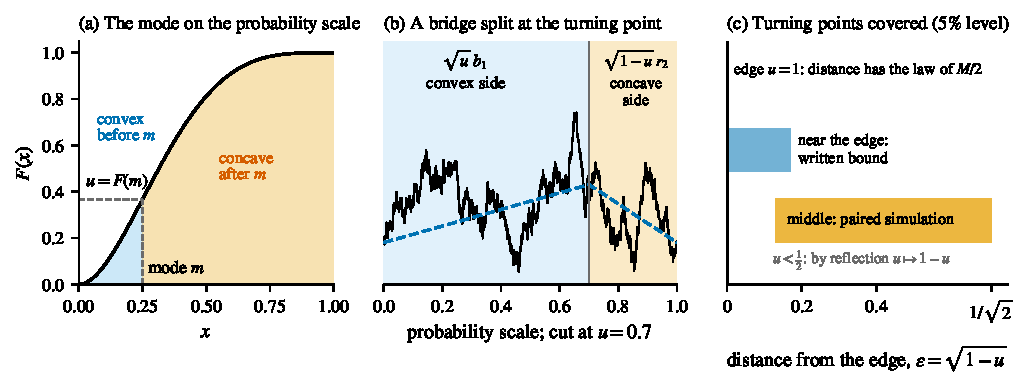
\includegraphics[width=\linewidth]{figs/fig7_dependency.pdf}
\caption{The geometry behind \cref{sec:worst}: every law reduces to a uniform sample with a fixed turning point, the bridge splits there into two independent halves, and two arguments together cover every turning point. (a) A unimodal distribution function curves upward before the mode $m$ and downward after it; on the probability scale the mode sits at $u=F(m)$. (b) One simulated Brownian bridge cut at $u=0.7$: after the dashed broken line is removed, the left piece is $\sqrt u\,b_1$ and the right piece is $\sqrt{1-u}\,r_2$, two independent bridges (\cref{lem:seam}); the fit must be convex on the left and concave on the right. (c) At the 5 percent level, the turning points near the edge are handled by a written bound and those in the middle by a paired simulation; the two ranges overlap, the edge itself gives the law of $M/2$, and reflection covers $u<\frac12$.}
\label{fig:dependency}
\end{figure}

We split the turning points into two overlapping ranges, as \cref{fig:dependency}(c) shows. Close to the edge, the two pieces of the bridge in \cref{lem:seam} are very unequal: the right piece is short, of scale $\varepsilon=\sqrt{1-u}$. There a written argument bounds $g(u,t')-g(1,t')$ from above by an explicit expression in published laws of Brownian functionals, including the description of the convex minorant of Brownian motion by Pitman and Uribe Bravo \cite{PUB12}, and interval arithmetic shows that the expression is negative throughout that range. Further from the edge no such expansion is accurate, and we compare each turning point directly with the edge on the same simulated pairs of bridges. For each pair we record whether the edge exceeds $t'$ while no turning point in a small cell does, or the reverse; the record is built so that its expected value is at least the largest rejection probability in the cell minus the one at the edge, so a negative expectation covers every turning point in the cell, not only a grid of them. A sign test in each cell shows that the edge wins by a wide margin. Reflection, $u\mapsto1-u$, covers turning points left of the middle.

The exact ranges, the number of cells and paths, and the error budget are listed in \cref{app:cert}. The probability that the two computations together certify a false statement is at most $1.1\cdot10^{-3}$ at each level.

\begin{theorem}[worst-case size; certified, conditional]\label{thm:worst}
Assume the quantile convergence of \cref{sec:setting}, the written lemmas behind \cref{thm:reduction} (\cref{lem:seam} and the proof in \cref{app:proofs}), and the four written lemmas behind the near-edge bound (\cref{app:cert}). On the event that the two certificates above and the bracket for $\qbar_\alpha$ are correct, both $\liminf_nS_n(\alpha)$ and $\limsup_nS_n(\alpha)$ lie in
\[
[40.45,\,46.22]\%\ \ (\alpha=10\%),\qquad[28.40,\,33.20]\%\ \ (\alpha=5\%),\qquad[12.67,\,16.79]\%\ \ (\alpha=1\%).
\]
\end{theorem}
\begin{proof}
Because $t'<\qbar_\alpha$, the uniform critical values satisfy $\sqrt n\,q_n(1-\alpha)>t'$ for all large $n$, so rejection implies $\sqrt nD_n>t'$. \Cref{thm:reduction} and the certified edge statement then give $\limsup_nS_n\le g(1,t')=1-F_M(2t')$. For the lower bound, $S_n$ is at least the rejection probability of any fixed law, so \cref{cor:lf}(b) gives $\liminf_nS_n\ge1-F_M(2\qbar_\alpha)\ge1-F_M(2q_+)$. The rigorous enclosure of $F_M$ turns both ends into the numbers shown.
\end{proof}

These intervals are the ones in \cref{tab:size} for fixed laws; we do not show that the two quantities are equal, only that both lie in the same intervals. Moving laws do not make the standard test worse in the limit by more than the width of these intervals, and the flat shoulder with a thin top comes within that width of the worst case. We do not claim that $\lim_nS_n$ exists, or that any law attains it.

The same machinery answers whether $c_\alpha$ also controls the worst-case size. At $t=c_\alpha$ an analogous computation certified, with joint confidence at least $0.99$, that $g(u,c_\alpha)<\alpha$ for $u\in[0.0159,0.9841]$ at 5 percent and $u\in[0.0176,0.9824]$ at 1 percent. A written near-edge theorem, checked in Lean given its published inputs, covers $u\in[0.9775,1)$. On the event that the certificate is correct, and conditional on the same lemmas, $\lim_n\sup_FP_F(\sqrt nD_n>c_\alpha)=\alpha$ at both levels: the corrected cutoff keeps its level uniformly over all continuous unimodal laws, in the limit.

\section{Finite samples}\label{sec:finite}

Limits describe large samples. This section answers two questions for the sample sizes people use: how large is the worst-case size of the standard test at a given $n$, and which cutoff keeps the level at that $n$. Every statement here is made at the listed values of $n$ only; we prove nothing about monotonicity in $n$.

\subsection{The size of the standard test}
At each of 21 sample sizes from $n=4$ to $n=1000$, and at the levels 10, 5 and 1 percent, we enclosed the worst-case size $S_n(\alpha)$ in an interval. The 63 intervals hold jointly with confidence at least $0.991$.

The lower end of each interval is witnessed by a specific unimodal law. We found the law by search, and then re-estimated its rejection rate on fresh random draws, so the search cannot bias the estimate; an exact binomial bound turns the estimate into a lower confidence limit.

The upper end comes from one computation on uniform samples, which by \cref{thm:envelope} covers every law at once. For each simulated uniform sample we bound its distance to $K_u$ over all turning points $u$, and the sample counts as non-rejecting only when a certified upper bound on that distance falls strictly below the cutoff.

\Cref{fig:worstsize} shows them. At every listed $n$ and level the size exceeds the nominal level. At $n=1000$ the 5 percent test has worst-case size between 28.0 and 34.2 percent, which agrees with the asymptotic interval of \cref{thm:worst}. At small $n$ the intervals are wide, 27 to 57 points for $n$ between 5 and 12, so the exact worst-case size there is not known. A simpler statement holds at every $n$: with the same joint confidence, the running example $W(0.1,0.005)$ is rejected more often than the nominal rate at each of the 997 integers from 4 to 1000 and at all three levels. At $n=50$, for example, its rejection rates are 3.9, 13.5 and 23.2 percent at the 1, 5 and 10 percent levels.

\begin{figure}[t]
\centering
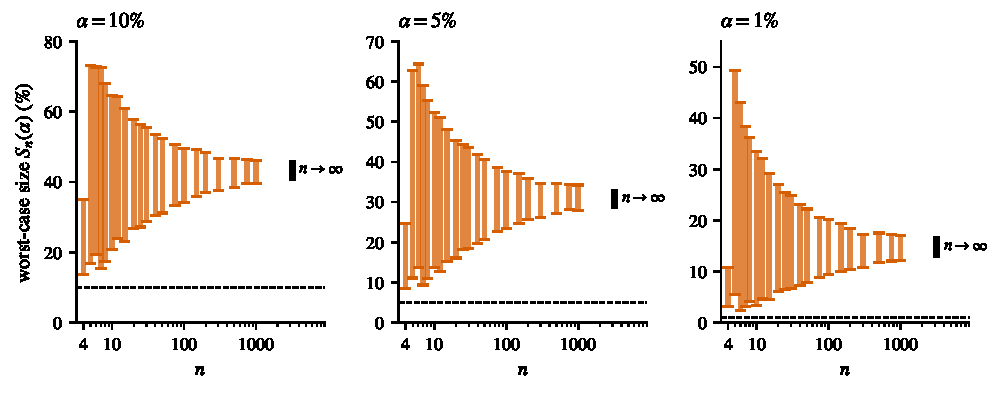
\includegraphics[width=\linewidth]{figs/fig4_worst_size.pdf}
\caption{The worst-case size of the standard dip test exceeds the nominal level at every sample size shown, and at $n=1000$ its enclosure overlaps the asymptotic interval. Orange bars: enclosures at 21 sample sizes. They hold jointly with confidence at least $0.991$, and their lower ends at $n=4$ are exact. Black bars: the asymptotic interval of \cref{thm:worst}. Dashed lines: nominal level.}
\label{fig:worstsize}
\end{figure}

\subsection{Certified cutoffs}
\Cref{thm:envelope} also turns the search for a valid cutoff into a computation on uniform samples. For a candidate cutoff $d$ at a given $n$ we simulate uniform samples, compute the distance to $K_u$ over each block of turning points by an exact linear program, and accept $d$ when the binomial upper bound on the exceedance rate is at most $\alpha$ in every block, after a Bonferroni correction over all candidates and sample sizes in the run. \Cref{tab:cutoffs} lists the result, and \cref{fig:cutoffs} compares the certified cutoffs with the uniform quantiles that the standard test uses.

\begin{table}[t]
\centering
\small
\caption{Certified dip cutoffs. Rejecting when $D_n\ge d$ has size at most $\alpha$ over all continuous unimodal laws at the listed $n$. Cutoffs are given on the scale $\sqrt n\,d$, except at $n=4$, where $d$ itself is shown with the certified bound on the size. The false-certification probability is at most $0.001$ for the first two rows and at most $0.02$ for the third.}
\label{tab:cutoffs}
\begin{tabular}{p{2.9cm}ccc}
\toprule
$n$ & $\alpha=10\%$ & $\alpha=5\%$ & $\alpha=1\%$ \\
\midrule
4 & $0.2335$ ($\le9.62\%$) & $0.2420$ ($\le4.62\%$) & $0.2488$ ($\le0.68\%$) \\
8 to 49, every $n$ & $\rho\times0.667$ & $\rho\times0.7313$ & $\rho\times0.8585$ \\
50, 100, 200, 400, 800, 1600 & & $0.7315$ & $0.86$ ($n\le800$); $0.87$ ($n=1600$) \\
\bottomrule
\end{tabular}
\par\smallskip
\raggedright\footnotesize For $8\le n\le49$ the certified cutoff is $\rho$ times the lower end of the bracket for $c_\alpha$, divided by $\sqrt n$. The factor $\rho$ was chosen from the fixed ladder $0.900,0.905,\dots,0.995$ by a rule set in the protocol; the certified values lie between $0.945$ and $0.995$ and depend on $n$ and $\alpha$, and the full list is in the supplement. In five of these 126 cases ($n=8,10,11$ at 1 percent and $n=9$ at 5 and 1 percent) the certified cutoff exceeds the largest possible dip (\cref{lem:maxdip}), so the test never rejects there.
\end{table}

\begin{figure}[t]
\centering
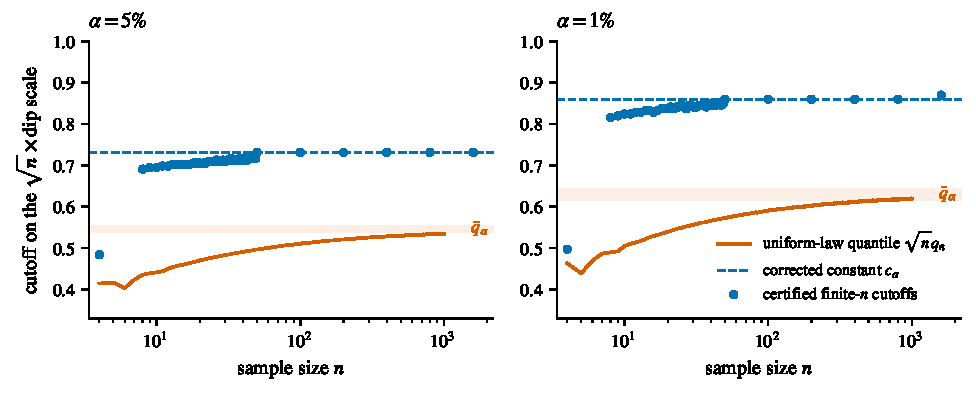
\includegraphics[width=\linewidth]{figs/fig5_cutoffs.pdf}
\caption{Valid cutoffs lie above the uniform quantiles that the standard test uses, at every sample size. Cutoffs are shown on the scale $\sqrt n\times$dip. Orange: the uniform quantile $\sqrt n\,q_n$ used by the standard test, rising towards $\qbar_\alpha$ (shaded bracket). Blue dashed: the corrected constant $c_\alpha$. Blue dots: certified cutoffs from \cref{tab:cutoffs}. At every $n$ shown, the certified cutoff lies above the uniform quantile.}
\label{fig:cutoffs}
\end{figure}

Three features of the table matter in practice. At $n=4$ the certified cutoffs lie just below $1/4$, the largest dip four points can have, while $c_\alpha/\sqrt4$ exceeds $1/4$ at every level, so the asymptotic cutoff could never reject at $n=4$. For $8\le n\le49$ the certified cutoffs lie a little below $c_\alpha/\sqrt n$, so each certified test rejects whenever the asymptotic one does and has at least its power; as a by-product, $c_\alpha/\sqrt n$ itself has size at most $\alpha$ at all 126 of these $(n,\alpha)$ pairs. At the six listed sizes from 50 to 1600, the rounded value $0.7315$ is certified at 5 percent. The best laws we found reach only 1.6 to 3.3 percent at that cutoff, so the certified cutoffs are valid but we do not claim that they are the smallest valid ones. Two cutoffs that are valid at every $n$ are already known, and both are larger: half the Kuiper distance of Davies and Kovac \cite{DK04}, $0.874/\sqrt n$ at 5 percent, and the Dvoretzky--Kiefer--Wolfowitz bound with Massart's constant \cite{Massart90}, $1.3582/\sqrt n$ at 5 percent and $1.6277/\sqrt n$ at 1 percent.

\subsection{Very small samples}
At $n=4$ the dip has a closed form. If $s_1,s_2,s_3$ are the gaps between the four ordered observations, Hartigan and Hartigan \cite[p.~73]{HH85} show that $D=T/(4(T+1))$ with $T=\max\{1,\,s_2/\max(s_1,s_3)\}$. Under the uniform law $P(T\ge r)=2/((r+1)(r+2))$ for $r>1$, so the exact uniform critical value is $q_4(1-\alpha)=r_\alpha/(4(r_\alpha+1))$, where $(r_\alpha+1)(r_\alpha+2)=2/\alpha$. For a step law the rejection probability is then the volume of a polytope, which we compute in rational arithmetic. For the running example the exact rates, truncated to four decimals, are $10.6639$, $5.5465$ and $1.2908$ percent at the 10, 5 and 1 percent levels, only a small excess at this sample size. Other laws do worse. Laws built from parts on widely separated scales give
\[
S_4(\alpha)\ \ge\ 13.7461,\ 8.5962,\ 3.2638\ \text{percent at}\ \alpha=10,\ 5,\ 1\ \text{percent},
\]
and we conjecture that these values are the exact worst case. The Monte Carlo upper bounds are 34.93, 24.60 and 10.70 percent. At $n=4$, then, the flat shoulder with a thin top is not the worst shape.

Small samples also have a hard ceiling on the dip, which explains the five cases in \cref{tab:cutoffs} where the certified test never rejects.

\begin{lemma}[largest possible dip]\label{lem:maxdip}
For every $n\ge1$ and every data set, ties allowed, $D(F_n)\le\lfloor n/2\rfloor/(2n)$. The bound is attained when $\lfloor n/2\rfloor$ points sit at one value and the rest at another.
\end{lemma}
\begin{proof}
Let $k=\lfloor n/2\rfloor$, $\varepsilon=k/(2n)$, let $m$ be the $(k+1)$-th order statistic and $R>0$ the sample range (if $R=0$ the dip is $0$). For $T\ge R$ let $G_T$ put mass $\varepsilon$ evenly on $[m-T,m]$, an atom $1-2\varepsilon$ at $m$, and mass $\varepsilon$ evenly on $[m,m+T]$; it is unimodal with mode $m$. Left of $m$ we have $F_n\le k/n=2\varepsilon$, and from $m$ on $F_n\ge(k+1)/n\ge1-2\varepsilon$, and comparing the two functions gives $\sup|F_n-G_T|\le\varepsilon(1+R/T)$. Let $T\to\infty$.
\end{proof}

The value $1/4$ for even $n$ is noted in Mächler's vignette \cite{Maechler}; the odd-$n$ value $(n-1)/(4n)$ is elementary, and we did not find it stated elsewhere.

\section{Power and practical use}\label{sec:practice}

\subsection{Power}
The corrected test and the standard test apply different cutoffs to the same statistic, so their rejection regions are nested and the corrected test never has more power. The question is how much power it gives up, and how it compares with other cutoffs that are also valid. We compared four constant cutoffs on the dip, on a preregistered panel of 37 laws with 50,000 samples per law and sample size, for $n$ from 50 to 12,800.

On the null laws of the panel the uniform calibration exceeded its nominal level at every $n$, with rejection rates as high as 30.7 percent at the 5 percent level and 13.7 percent at the 1 percent level. The corrected cutoff $c_\alpha/\sqrt n$ stayed within the preregistered tolerance on every null law: the upper end of each 95 percent interval was at most $\alpha$ plus 0.5 points at the 5 percent level and $\alpha$ plus 0.25 points at the 1 percent level. Its largest rates were 4.53 and 0.90 percent, and they rose towards $\alpha$ from below as $n$ grew. Of the three cutoffs that stayed within tolerance, the corrected one is the smallest and therefore the most powerful. On the 14 alternatives whose power reached 80 percent inside the range of $n$ we simulated, half the Kuiper distance needed 1.35 to 1.55 times as many observations as $c_\alpha$, and the DKW bound 3.3 to 3.7 times. Against the uniform calibration, whose size is not controlled, the corrected test needs about twice the sample size. \Cref{fig:power} shows two symmetric normal mixtures.

\begin{figure}[t]
\centering
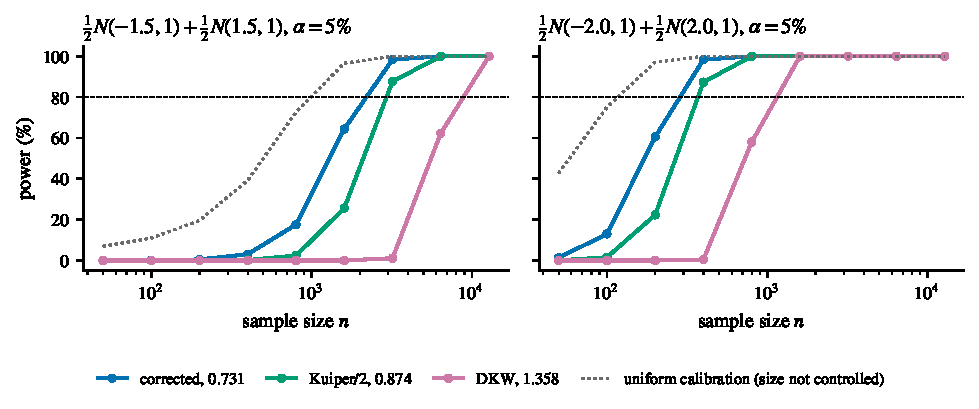
\includegraphics[width=\linewidth]{figs/fig6_power.pdf}
\caption{Among the cutoffs that keep the level, the corrected cutoff reaches high power at the smallest sample size. Power at the 5 percent level for two symmetric normal mixtures, with $50{,}000$ samples per point. Blue: the corrected cutoff $c_\alpha/\sqrt n$, asymptotically valid on $\cC$ and within tolerance on every null law of the panel. Green and purple: half the Kuiper distance and the DKW bound, valid at every $n$. Grey dotted: the uniform calibration, whose size is not controlled, shown for reference only. The dashed line marks 80 percent power.}
\label{fig:power}
\end{figure}

For small samples we compared the certified cutoffs of \cref{tab:cutoffs} with global tests of unimodality derived from the multiscale methods of Dümbgen and Walther \cite{DW08} and Rufibach and Walther \cite{RW10}. The panel had 16 bimodal laws, 11 sample sizes from 8 to 49, three levels and $10^4$ shared samples per case. The dip with certified cutoffs rejected more often in 81 to 128 of the 176 cases per comparator and level, judged by pointwise 99 percent intervals, and after a Holm correction no comparator did significantly better in any case. The multiscale methods also locate modes, which the dip does not, and we did not compare that ability. With its default grid the block criterion cannot reject at all for $n<23$.

\subsection{Data that produce flat shoulders}
The failure needs a density that is flat over a long stretch and then rises sharply. This happens when most of the data are close to uniform and a small part piles up at one end. Collections of $p$-values are the clearest example. In an exploratory screen, mixtures of uniform null $p$-values with a small fraction of strong signals near zero were rejected 11 to 22 percent of the time by the nominal 5 percent test, for $n$ between 200 and 800. The same screen found no material excess for curved pile-ups such as a censored normal, a top-coded Beta law or a zero-inflated law, so the failure does not extend to every pile-up. Among 180 published applications of the dip that we sampled, one applied it to $p$-values \cite{Roy26}.

Clustering methods inherit the calibration of the dip they call. In simulation, changing only the critical values inside the UniDip and SkinnyDip procedures \cite{Maurus16}, from the uniform table to $c_\alpha/\sqrt n$, cut the probability of splitting a unimodal feature with a flat part or a pile-up into two clusters from 13 to 29 percent down to 1 to 3 percent. The change also costs power: for one three-component mixture at $n=500$ the detection rate fell from 56 to 8.5 percent.

Two other calibrations did not solve the problem. Our implementation of the calibrated dip of Cheng and Hall \cite{CH98}, which reproduces their published table to within 1.2 points, rejected the uniform law in 30 to 81 percent of samples and $W(0.1,0.005)$ in 50 to 100 percent at the 5 percent level, for $n$ between 50 and 12,800. These laws lie outside the smoothness conditions of that method, and Cheng and Hall \cite{CH99} warned about shoulders themselves. A small neural network trained to interpolate between the uniform and the corrected cutoffs passed an internal audit, but a targeted search then found unimodal laws at which it rejected 16.9 percent of samples at the 5 percent level.

\subsection{Recommendations}
\noindent\fbox{\parbox{\dimexpr\linewidth-2\fboxsep-2\fboxrule}{\setlength{\parskip}{3pt}
\textbf{Which cutoff to use.}
\begin{itemize}[leftmargin=*,topsep=2pt]
\item $n\ge50$: reject unimodality at the 5 percent level when $\sqrt nD_n\ge0.7315$, and at the 1 percent level when $\sqrt nD_n\ge0.86$ ($0.87$ at $n=1600$). These cutoffs carry a finite-sample certificate only at the six sample sizes of \cref{tab:cutoffs}; at other $n\ge50$ they rest on the limit results, which keep the level on $\cC$ as $n\to\infty$.
\item $n=4$ and $8\le n\le49$: use the certified cutoffs of \cref{tab:cutoffs}.
\item Report a $p$-value from the uniform table only as a description of the data, not as evidence at a stated level.
\end{itemize}}}

\vspace{10pt}\noindent A user who prefers power to a size guarantee should know what the uniform table buys: false alarms on up to about a third of unimodal samples at the nominal 5 percent level.

\section{Discussion}\label{sec:discussion}

The claim that the uniform law is the worst case for the dip fails once flat stretches are allowed. When the density can stay flat over a long interval and then rise sharply, the fit loses the freedom to choose its turning point on that interval, and the dip stops behaving like the uniform limit $D(B)$ and starts behaving like $M/2$, half the largest gap between a Brownian bridge and its convex minorant. Everything else in the paper measures the consequences of that change of limit. For fixed laws, the standard 5 percent test can reject about 30 percent of unimodal samples in large samples, and no law in the class $\cC$ pushes it further. Replacing the uniform cutoff by $c_\alpha/\sqrt n$ restores the level in the limit, and no deterministic sequence of cutoffs with a smaller limit does. When the worst law is allowed to change with $n$, the worst-case size lies in the same certified intervals. The $n=4$ counterexample of Hartigan and Hartigan was an early view of the same effect.

\paragraph{Limitations.} Three points affect how far the results can be relied on.
\begin{itemize}[leftmargin=*]
\item \emph{Conditional results.} \Cref{thm:worst} and the uniform statement about $c_\alpha$ in \cref{sec:worst} rest on written lemmas, on published laws, and on certificates with stated error probabilities. They are not theorems in the usual sense.
\item \emph{Width.} The size intervals are about five points wide at the 5 percent level, and almost all of that width comes from the bracket for $\qbar_\alpha$. A tighter bracket would narrow them without new theory.
\item \emph{Scope.} \Cref{thm:upper} covers laws with bounded support and a finite density at the mode. Laws outside $\cC$, such as the $p$-value mixtures of \cref{sec:practice}, are covered only by \cref{thm:envelope,thm:reduction}. All results assume independent observations from a continuous law.
\end{itemize}

\paragraph{Open questions.} Is the turning point at the right end of the probability scale always the worst one, that is, $g(u,t)\le g(1,t)$ for every $t$ and every $u$? A proof would replace the computation of \cref{sec:worst}. What is the worst-case size at small $n$, where our intervals are wide, and is it attained by laws built from parts on separated scales, as at $n=4$? And how should the dip be calibrated when observations are dependent, as in time series, where the empirical process has a different limit and the shoulder mechanism may be stronger or weaker?

\section*{Declaration of generative AI use}
The author used Claude, a generative AI model developed by Anthropic, extensively in writing and testing the code, and developing the Lean formalisation. Every result reported here was checked against the deposited computations and, where stated, the Lean kernel, as described in the paper. The author takes full responsibility for the content.


\begin{thebibliography}{99}\small

\bibitem{BF11} F.~Balabdaoui and K.~Filali. Efficient computation of the cdf of the maximal difference between Brownian bridge and its concave majorant. \emph{Journal of Statistical Computation and Simulation}, doi:10.1080/00949655.2010.534481. Preprint arXiv:1005.1307.

\bibitem{BP11} F.~Balabdaoui and J.~Pitman. The distribution of the maximal difference between a Brownian bridge and its concave majorant. \emph{Bernoulli}, 17(1), 2011. doi:10.3150/10-BEJ280.

\bibitem{Bauer23} L.~G.~M. Bauer, C.~Leiber, C.~Böhm and C.~Plant. Extension of the dip-test repertoire: efficient and differentiable p-value calculation for clustering. In \emph{Proceedings of the 2023 SIAM International Conference on Data Mining}, 109--117, 2023.

\bibitem{Beare21} B.~K. Beare. Least favourability of the uniform distribution for tests of the concavity of a distribution function. \emph{Stat}, 10(1):e376, 2021.

\bibitem{Carolan02} C.~A. Carolan. The least concave majorant of the empirical distribution function. \emph{Canadian Journal of Statistics}, 30:317--328, 2002.

\bibitem{CD99} C.~A. Carolan and R.~Dykstra. Asymptotic behavior of the Grenander estimator at density flat regions. \emph{Canadian Journal of Statistics}, 27(3):557--566, 1999.

\bibitem{BF17} B.~K. Beare and Z.~Fang. Weak convergence of the least concave majorant of estimators for a concave distribution function. \emph{Electronic Journal of Statistics}, 11(2):3841--3870, 2017.

\bibitem{Billingsley99} P.~Billingsley. \emph{Convergence of Probability Measures}, 2nd edition. Wiley, 1999.

\bibitem{CH98} M.-Y. Cheng and P.~Hall. Calibrating the excess mass and dip tests of modality. \emph{Journal of the Royal Statistical Society, Series B}, 60(3):579--589, 1998.

\bibitem{CH99} M.-Y. Cheng and P.~Hall. Mode testing in difficult cases. \emph{The Annals of Statistics}, 27(4):1294--1315, 1999.

\bibitem{DK04} P.~L. Davies and A.~Kovac. Densities, spectral densities and modality. \emph{The Annals of Statistics}, 32(3):1093--1136, 2004.

\bibitem{Lean4} L.~de Moura and S.~Ullrich. The Lean 4 theorem prover and programming language. In \emph{Automated Deduction, CADE 28}, Lecture Notes in Computer Science 12699, 625--635, 2021.

\bibitem{DW08} L.~Dümbgen and G.~Walther. Multiscale inference about a density. \emph{The Annals of Statistics}, 36(4):1758--1785, 2008.

\bibitem{Hartigan00} J.~A. Hartigan. Testing for antimodes. In W.~Gaul, O.~Opitz and M.~Schader (eds), \emph{Data Analysis: Scientific Modeling and Practical Application}, 169--181. Springer, 2000.

\bibitem{HH85} J.~A. Hartigan and P.~M. Hartigan. The dip test of unimodality. \emph{The Annals of Statistics}, 13(1):70--84, 1985.

\bibitem{Arb} F.~Johansson. Arb: efficient arbitrary-precision midpoint-radius interval arithmetic. \emph{IEEE Transactions on Computers}, 2017.

\bibitem{KMT75} J.~Komlós, P.~Major and G.~Tusnády. An approximation of partial sums of independent RV's and the sample DF.~I. \emph{Zeitschrift für Wahrscheinlichkeitstheorie und verwandte Gebiete}, 32:111--131, 1975.

\bibitem{KL08} V.~N. Kulikov and H.~P. Lopuhaä. Distribution of global measures of deviation between the empirical distribution function and its concave majorant. \emph{Journal of Theoretical Probability}, 21:356--377, 2008.

\bibitem{Maechler} M.~Mächler. Dip test distributions, P-values, and other explorations. Vignette of the R package \texttt{diptest}, version 0.77-2, CRAN.

\bibitem{Massart90} P.~Massart. The tight constant in the Dvoretzky--Kiefer--Wolfowitz inequality. \emph{The Annals of Probability}, 18(3):1269--1283, 1990.

\bibitem{Mathlib} The mathlib Community. The Lean mathematical library. In \emph{Proceedings of the 9th ACM SIGPLAN International Conference on Certified Programs and Proofs}, 367--381, 2020.

\bibitem{MP09} A.~Maurer and M.~Pontil. Empirical Bernstein bounds and sample variance penalization. In \emph{Proceedings of the 22nd Conference on Learning Theory (COLT)}, 2009.

\bibitem{Maurus16} S.~Maurus and C.~Plant. Skinny-dip: clustering in a sea of noise. In \emph{Proceedings of the 22nd ACM SIGKDD International Conference on Knowledge Discovery and Data Mining}, 1055--1064, 2016.

\bibitem{Mueller92} D.~W. Müller. The excess mass approach in statistics. Beiträge zur Statistik Nr.~3, Institut für Angewandte Mathematik, Universität Heidelberg, 1992.

\bibitem{MS91} D.~W. Müller and G.~Sawitzki. Excess mass estimates and tests for multimodality. \emph{Journal of the American Statistical Association}, 86(415):738--746, 1991.

\bibitem{PUB12} J.~Pitman and G.~Uribe Bravo. The convex minorant of a Lévy process. \emph{The Annals of Probability}, 40(4), 2012. doi:10.1214/11-AOP658.

\bibitem{Polonik95} W.~Polonik. Measuring mass concentrations and estimating density contour clusters: an excess mass approach. \emph{The Annals of Statistics}, 23(3):855--881, 1995.

\bibitem{Roy26} A.~Roychowdhury. Reconnection-driven state transitions in flat spectrum radio quasars. \emph{The Astrophysical Journal}, 1002:175, 2026.

\bibitem{RW10} K.~Rufibach and G.~Walther. The block criterion for multiscale inference about a density, with applications to other multiscale problems. \emph{Journal of Computational and Graphical Statistics}, 19(1), 2010. doi:10.1198/jcgs.2009.07071.

\end{thebibliography}


\appendix
\section{Proofs}\label{app:proofs}

Each proof below starts with what it shows and the idea behind it, and then goes through numbered steps. Each step does one thing. The proofs of \cref{prop:blocks} and \cref{thm:upper} give the full construction; the longer bookkeeping for those two (exact constants in the error terms) is in the supplementary notes.

\subsection{Three facts used throughout}
Let $I\subseteq J$ be intervals and $h,h_1,h_2$ bounded functions.
\begin{itemize}[leftmargin=*]
\item \emph{Restriction.} $V_I(h)\le V_J(h)$, because a convex function on $J$ is also convex on $I$.
\item \emph{Lines and scale.} Adding a linear function to $h$ does not change $V_I(h)$, and $V_I(ch)=cV_I(h)$ for $c>0$. Adding a line keeps a function convex, and scaling by $c>0$ keeps it convex.
\item \emph{Lipschitz.} $|V_I(h_1)-V_I(h_2)|\le\sup_I|h_1-h_2|$. Any fit to $h_1$ is a fit to $h_2$ with at most that much more error.
\end{itemize}
The same three facts hold for the concave distance $C_I$ and for the dip $D$, and all of these distances are unchanged by an increasing affine change of the variable.

\subsection{Three lemmas}

\begin{lemma}[bridge pieces]\label{lem:pieces}
For $0<s\le1$, the process $u\mapsto B(su)-uB(s)$, $u\in[0,1]$, has the law of $\sqrt s\,B'$, where $B'$ is a standard Brownian bridge independent of $B(s)$. Pieces of $B$ over disjoint intervals, each with its chord removed, are independent scaled bridges, and they are independent of the values of $B$ at the endpoints. In particular $V_{[0,s]}(B)$ has the law of $\sqrt s\,M/2$.
\end{lemma}

\goal{that a piece of a bridge looks like a smaller bridge, and that different pieces do not interact.}
\idea{all the processes involved are centred Gaussian, so independence and the law follow from covariances.}

\begin{proof}
\begin{steps}
\item \emph{Covariance with the endpoint value.} For $b(u)=B(su)-uB(s)$,
\[
\operatorname{Cov}\bigl(b(u),B(s)\bigr)=su(1-s)-us(1-s)=0 .
\]
\item \emph{Covariance of the piece.} For $u\le u'$, $\operatorname{Cov}(b(u),b(u'))=s\,u(1-u')$, which is the covariance of $\sqrt s$ times a standard bridge.
\item \emph{Disjoint pieces.} The same computation gives zero covariance between pieces over disjoint intervals, and between each piece and the endpoint values. Jointly Gaussian variables with zero covariance are independent.
\item \emph{The convex distance.} Removing the chord does not change $V$ (it is a linear function), scaling multiplies $V$ by $\sqrt s$, and $V(B')$ has the law of $M/2$ by \cref{lem:halfgap}.\qedhere
\end{steps}
\end{proof}

\begin{lemma}[localisation]\label{lem:local}
Let $F$ have a pinned shoulder on $[0,L]$, fix $\delta\in(0,L)$, and let $\kappa_\delta=C_{[L-\delta,1]}(F)>0$ be as in \cref{def:shoulder}. On the event $E_n=\{\sup|F_n-F|<\kappa_\delta/2\}$,
\[
D(F_n)\ \ge\ V_{[0,L-\delta]}(F_n),
\]
and $P(E_n)\to1$.
\end{lemma}

\goal{that once the sample is close to $F$, every good unimodal fit turns to the right of the shoulder, so the dip is at least the convex distance on the shoulder.}
\idea{a fit that turned inside the shoulder would have to be concave on $[L-\delta,1]$, and the pin keeps every such function far from the data.}

\begin{proof}
Write $e=\sup|F_n-F|$ and assume $e<\kappa_\delta/2$.
\begin{steps}
\item \emph{The dip is small.} $F$ itself is unimodal, so $D(F_n)\le e$.
\item \emph{Fits that turn early are far away.} A unimodal fit whose turning point is at most $L-\delta$ is concave on $[L-\delta,1]$. Its distance to $F_n$ is therefore at least
\[
C_{[L-\delta,1]}(F_n)\ \ge\ \kappa_\delta-e\ >\ e .
\]
\item \emph{Good fits turn late.} Take fits $g_k$ whose distance to $F_n$ decreases to $D(F_n)\le e$. By Step 2 these fits eventually turn to the right of $L-\delta$, so they are convex on $[0,L-\delta]$, and their distance to $F_n$ is at least $V_{[0,L-\delta]}(F_n)$. Letting $k\to\infty$ gives the inequality. We never need an optimal fit to exist.
\item \emph{The event is likely.} $P(E_n)\to1$ by the Glivenko--Cantelli theorem.\qedhere
\end{steps}
\end{proof}

\begin{lemma}[seam decoupling]\label{lem:seam}
Fix $u\in(0,1)$ and put
\[
b_1(s)=\frac{B(us)-sB(u)}{\sqrt u},\qquad r_2(s)=\frac{B\bigl(u+(1-u)s\bigr)-(1-s)B(u)}{\sqrt{1-u}},\qquad s\in[0,1].
\]
Then $b_1$, $r_2$ and $B(u)$ are independent, and $b_1$ and $r_2$ are standard bridges. Moreover $d(B,K_u)=d(H_u,K_{1/2})$, where $H_u(s)=\sqrt u\,b_1(2s)$ for $s\le\frac12$ and $H_u(s)=\sqrt{1-u}\,r_2(2s-1)$ for $s\ge\frac12$. At the edge put $H_1(s)=b_1(2s)$ for $s\le\frac12$ and $H_1(s)=0$ for $s\ge\frac12$; then $d(H_1,K_{1/2})=V(b_1)$, which has the law of $d(B,K_1)$. With one fixed pair $(b_1,r_2)$, the formula for $H_u$ defines all $u\in[\frac12,1]$ at once, each with the correct law, and $u\mapsto H_u$ is continuous in the supremum norm.
\end{lemma}

\goal{that cutting the bridge at the turning point $u$ leaves two independent bridges, and that the distance to $K_u$ depends only on them.}

\begin{proof}
\begin{steps}
\item \emph{Independence.} The covariance computation is the one in \cref{lem:pieces}.
\item \emph{Removing the value at $u$.} The broken line through $(0,0)$, $(u,B(u))$ and $(1,0)$ is linear on each side of $u$. Adding it to a member of $K_u$ gives another member, so subtracting it from $B$ does not change the distance to $K_u$.
\item \emph{Moving the turning point to $\frac12$.} The increasing affine maps $[0,\frac12]\to[0,u]$ and $[\frac12,1]\to[u,1]$ carry $K_u$ onto $K_{1/2}$ and keep supremum distances.\qedhere
\end{steps}
\end{proof}

\subsection{Proof of \cref{thm:shoulder} (pinned shoulders)}

\goal{that the dip of a sample from a law with a pinned shoulder of mass $p$ is, in the limit, at least $\sqrt p\,M/2$.}
\idea{on the shoulder the fit must be convex (\cref{lem:local}); there $F$ is a line, so the convex distance of the data is the convex distance of the empirical fluctuation, which converges to a piece of a Brownian bridge.}

\begin{proof}
Fix $\delta\in(0,L)$ and write $J=[0,L-\delta]$.
\begin{steps}
\item \emph{Remove $F$.} $F$ is linear on $J$, and adding a line does not change $V_J$, so
\[
\sqrt n\,V_J(F_n)=V_J\bigl(\sqrt n(F_n-F)\bigr).
\]
\item \emph{Pass to the limit.} $V_J$ is Lipschitz for the supremum distance, and $\sqrt n(F_n-F)$ converges in law to $B\circ F$ by Donsker's theorem. By the continuous mapping theorem, $\sqrt nV_J(F_n)$ converges in law to $V_J(B\circ F)$.
\item \emph{Identify the limit.} After the change of variable $u=F(x)$, $V_J(B\circ F)=V_{[0,p_\delta]}(B)$ with $p_\delta=F(L-\delta)$. By \cref{lem:pieces} this has the law of $\sqrt{p_\delta}\,M/2$.
\item \emph{Combine with localisation.} \Cref{lem:local} says $\sqrt nD_n\ge\sqrt nV_J(F_n)$ on an event of probability tending to one. The portmanteau theorem for the open set $(t,\infty)$ then gives
\[
\liminf_n P\bigl(\sqrt nD_n>t\bigr)\ \ge\ P\bigl(\sqrt{p_\delta}\,M/2>t\bigr).
\]
\item \emph{Let $\delta\to0$.} As $\delta$ decreases, $p_\delta$ increases to $p$, and the events $\{\sqrt{p_\delta}\,M/2>t\}$ increase to $\{\sqrt p\,M/2>t\}$.\qedhere
\end{steps}
\end{proof}

\emph{Proof of \cref{cor:shoulder}.} Fix $\eta>0$. Quantile convergence gives $\sqrt n\,q_n(1-\alpha)<\qbar_\alpha+\eta$ for all large $n$, so then $\{\sqrt nD_n>\qbar_\alpha+\eta\}\subseteq\{D_n\ge q_n(1-\alpha)\}$. The theorem at $t=\qbar_\alpha+\eta$ gives a limiting rejection rate of at least $1-F_M\bigl(2(\qbar_\alpha+\eta)/\sqrt p\bigr)$, and letting $\eta\to0$ gives the corollary, because $F_M$ is continuous.

\subsection{Proof of \cref{thm:fail} (the uniform calibration fails)}

\goal{that for every $\alpha$ some fixed two-step law is rejected with limiting probability above $\alpha$, using no numerical facts.}
\idea{as the shoulder mass tends to one, \cref{thm:shoulder} pushes the rejection rate up to $P(V(B)>q)$, while the uniform cutoff $q$ was built for $D(B)$. Since $D(B)\le V(B)$, it is enough to show that $V(B)$ is strictly larger than $D(B)$ with positive probability, in a way that crosses $q$.}

\begin{proof}
Let $H$ be the distribution function of $D(B)$ and let $q^+=\inf\{x:H(x)>1-\alpha\}$ be its upper $(1-\alpha)$ quantile.
\begin{steps}
\item \emph{The cutoff is positive.} A uniform limit of functions that are convex and then concave is again convex and then concave, so it is differentiable almost everywhere. A Brownian bridge is almost surely nowhere differentiable, so $D(B)>0$ almost surely. Hence $H(0)=0$ and $q^+>0$.
\item \emph{Rejection above any level beyond $q^+$.} Take a continuity point $x>q^+$ of $H$. Then $H(x)>1-\alpha$, and since $P_U(\sqrt nD_n\le x)\to H(x)$ under the uniform law, eventually $\sqrt n\,q_n(\alpha)\le x$. From then on $\{\sqrt nD_n>x\}\subseteq\{D_n>q_n(\alpha)\}$.
\item \emph{Reduce to one bridge.} By \cref{thm:shoulder} with $p=1-w$, the limiting rejection rate under $W(w,\varepsilon)$ is at least $P(\sqrt{1-w}\,V(B)>x)$. Letting $x$ decrease to $q^+$ through continuity points, and then letting $w$ decrease to $0$, shows that it is enough to prove
\[
P\bigl(V(B)>q^+\bigr)>\alpha .
\]
Some small fixed $w$, with any $0<\varepsilon<w$, then gives the theorem.
\item \emph{$V(B)$ has no atoms.} We show that $P(V(B)=q)=0$ for every $q>0$. For a continuous $h$, $2V(h)$ is the supremum of the chord defect $h(t)-[(b-t)h(a)+(t-a)h(b)]/(b-a)$ over $0\le a<t<b\le1$; the defect extends continuously by $0$ to degenerate triples, so on the compact set of triples the supremum is attained, and when it is positive it is attained at a non-degenerate triple. Let $f_0(t)=t(1-t)$, $Z=6\int_0^1B$ and $R=B-Zf_0$. A covariance computation shows that $Z$ is a non-degenerate Gaussian variable independent of $R$. The chord defect of $f_0$ is $(t-a)(b-t)>0$, so $z\mapsto V(R+zf_0)$ is strictly increasing wherever it is positive. Each level $q>0$ is therefore reached for at most one value of $z$, and conditioning on $R$ gives $P(V(B)=q)=0$.
\item \emph{Split the event.} A convex function is an admissible unimodal fit, so $D(B)\le V(B)$ on every path. Since $H(q^+-)\le1-\alpha$, we have $P(D(B)\ge q^+)\ge\alpha$. Using Step 4,
\[
P\bigl(V(B)>q^+\bigr)\ \ge\ P\bigl(D(B)\ge q^+\bigr)+P\bigl(V(B)>q^+>D(B)\bigr)\ \ge\ \alpha+P\bigl(V(B)>q^+>D(B)\bigr).
\]
\item \emph{The last probability is positive.} Choose $0<\eta<q^+$ and $K$ with $K/8>q^++\eta$, and let $f(u)=Ku(1-u)$. This arch is concave, so $C(f)=0$, and its convex distance is $V(f)=K/8$. A Brownian bridge comes within $\eta$ of $f$ with positive probability, and on that event the Lipschitz property gives $V(B)>q^+$ and $D(B)\le C(B)<\eta<q^+$.\qedhere
\end{steps}
\end{proof}

\subsection{Proof of \cref{prop:blocks} (step densities)}

\goal{the exact limit of $\sqrt nD_n$ for a unimodal step density.}
\idea{perturb $F$ by a small multiple $r$ of a continuous function $h$ and find the first-order change of the dip. On each block left of the mode the fit must be convex, on each block right of it concave, and on the modal block it may turn. The difficulty is to join the separate fits into one unimodal function without losing anything.}

For a continuous $h$ with $h(0)=h(1)=0$, write $\tau_i(h)$ for the convex distance of $h$ on block $i$ if the block lies left of the mode, the concave distance if it lies right of the mode, and the dip of $h$ restricted to the block if it is the modal block (with the turning point allowed anywhere in the block). The claim is
\[
\lim_{r\to0}\frac{D(F+rh_r)}{r}=\max_i\tau_i(h)\qquad\text{whenever }h_r\to h\text{ uniformly}.
\]
By the Lipschitz fact we may take $h_r=h$. Two quantities control the join in the upper bound below. The distance $\eta=\sqrt r$ keeps the turning point of the modal fit away from the ends of the modal block, which leaves room to hand over from one piece to the next; it is large compared with $r$ but tends to zero. The gap $\Delta$ between adjacent heights must exceed $2rK$, so that each straight-line extension of a piece falls away from $F$ outside its own block.

\begin{proof}
\begin{steps}
\item \emph{Lower bound.} $F$ is linear on each block, so on the modal block the dip of $F+rh$ is $r$ times the dip of $h$, and every unimodal fit restricted to that block is admissible there. For a block left of the mode, $F$ has a convex kink at the block's right end. The argument of \cref{lem:local} shows that, once $r$ is small, good fits turn to the right of that kink, so $D(F+rh)\ge r$ times the convex distance of $h$ on the block shortened by $\delta$. Letting $\delta\to0$ gives $\tau_i(h)$. Blocks right of the mode are the mirror image.
\item \emph{Upper bound: the pieces.} Replace $h$ by a $K$-Lipschitz function within $\epsilon'$ of it and let $d=\max_i\tau_i$ for that function. On each block take a $K$-Lipschitz fit attaining the block's distance: convex on the left blocks, concave on the right blocks, and convex-then-concave on the modal block with turning point $\mu$. Move $\mu$ at least $\eta=\sqrt r$ away from the ends of the modal block; this costs at most $K\eta$.
\item \emph{Upper bound: the join.} Extend each convex piece $F+rg_i$ beyond its block by lines whose slopes differ from the block's density by $rK$. On $[0,\mu]$ take the largest of the convex pieces and on $[\mu,1]$ the smallest of the concave ones. Adjacent densities differ by a fixed amount $\Delta$, larger than $2rK$ for small $r$, so each extension stays within $r(d+\epsilon'+K\eta)$ of $F+rh$ outside its block. At $\mu$ the modal pieces exceed the others by $(\Delta-2rK)\eta-O(r)>0$, so the joined function is unimodal with turning point $\mu$, and its distance to $F+rh$ is at most $r(d+\epsilon'+K\eta)$. Let $r\to0$ and then $\epsilon'\to0$.
\item \emph{The limit law.} On a Skorohod representation in $D[0,1]$ with the $J_1$ topology \cite{Billingsley99}, $h_n=\sqrt n(F_n-F)\to B\circ F$ uniformly almost surely. Steps 1 to 3 with $r=n^{-1/2}$ give $\sqrt nD(F_n)\to\max_i\tau_i(B\circ F)$. On block $i$, $B\circ F$ is a bridge over a probability interval of length $p_i$, and with chords removed these pieces are independent scaled bridges by \cref{lem:pieces}.\qedhere
\end{steps}
\end{proof}

Step 3 needs a fixed gap $\Delta$ between adjacent heights. If two heights differ only by order $r$, the two blocks act as one shoulder: for three equal blocks with densities $\frac12\mp r\kappa/2$ and $2$, and a suitable piecewise linear $h$, every separate block term is zero while $D(F_r+rh)/r$ has a positive limit.

\subsection{Proof of \cref{thm:upper} (upper bound)}

\goal{that for every law in $\cC$ the limit of $\sqrt nD_n$ is no larger than $M/2$ in distribution.}
\idea{where $F$ is strictly curved it bends away from its tangent lines quadratically, and that curvature absorbs a perturbation of size $r$ at no first-order cost; only the flat stretches, where $F$ is a straight line, make the fit pay for the perturbation. So we bound the first-order change of the dip by the distances of $h$ on the flat stretches, and then compare all of those with the convex distance of one Brownian path. As in \cref{prop:blocks}, the work is in joining the left and right fits at the mode, and a general law forces us to treat three shapes of mode separately.}

Write $P=[m_1,m_2]$ for the modal set. Let $T_F(h)$ be the largest of three numbers: the supremum of the convex distances of $h$ over the maximal flat stretches inside $[0,m_1]$, the dip of $h$ on $P$ (zero if $m_1=m_2$), and the supremum of the concave distances over the maximal flat stretches inside $[m_2,1]$. There may be countably many stretches, so these are suprema. The deterministic claim is
\[
\limsup_{r\to0}\frac{D(F+rh_r)}{r}\ \le\ T_F(h)\qquad\text{whenever }h_r\to h\text{ uniformly}.
\]
After an approximation that changes both sides by at most $\epsilon$, we may take $h_r=h$ with $h$ smooth and $|h'|\le K$. Write $F_r=F+rh$.

\paragraph{Three tools.}
\begin{enumerate}[label=(T\arabic*),leftmargin=*,itemsep=4pt]
\item \emph{Seam shift.} If $g_1$ is convex on $[0,\mu]$, $g_2$ is concave on $[\mu,1]$, both are within $e$ of $F_r$, and $g_1(\mu)-g_2(\mu)\le\delta$, then $D(F_r)\le e+\max(\delta,0)/2$. Lowering $g_1$ and raising $g_2$ by half the mismatch joins them.
\item \emph{Endpoint fit.} For a continuous $\psi$ on $[0,a]$, the function $\GCM(\psi)+V_{[0,a]}(\psi)$ is convex, lies within $V_{[0,a]}(\psi)$ of $\psi$, and has left slope at $a$ at most any $s$ with $\psi(a)-\psi(x)\le s(a-x)$ for all $x<a$. This controls how steeply a fit leaves an interval.
\item \emph{One-sided limit.} If $F$ is convex on an interval $I$, then $V_I(F+rh)/r$ converges to the largest convex distance of $h$ over the maximal flat stretches inside $I$. No curvature condition is needed, and the stretches may accumulate. This is a form of the directional derivative of Beare and Fang \cite{BF17}; the concave case is the mirror image.
\end{enumerate}

\paragraph{Case A: a modal interval ($m_1<m_2$).} Let $f$ be the monotone one-sided density, $f^*$ its value on $P$, $\ell_P$ the linear function equal to $F$ on $P$, and $T_L$, $T_R$ the left and right parts of $T_F(h)$. 

The plan is to use the best turning fit on the flat top $P$, the best convex fit on everything to its left, and the mirror on the right, and to make sure that the left fit hands over to the top fit before the turning point is reached. Four constants control this. The width $\eta$ keeps the turning point of the top fit at least $\eta$ inside $P$, so that there is room to hand over. The factor $\lambda<1$ squeezes the top fit slightly, which makes its end slopes finite. The constant $M'$ decides how far the density must fall below its peak value $f^*$ before we stop using the top fit; it defines a window around $P$ that shrinks to $P$ as $r\to0$. The condition that $(M'-2K)\eta$ is large guarantees that, at the turning point, the extended left fit lies well below the top fit, so taking the larger of the two selects the top fit there. The order of choices matters: first $\epsilon$ and $h$ (which fix the Lipschitz constant $K$), then $\eta$ with $2\eta<m_2-m_1$, then the top fit, then $M'$, and only then $r\to0$.
\begin{steps}
\item \emph{Modal fit.} Take a convex-then-concave fit $\varphi$ of $h$ on $P$ with error at most $D_P(h)+\epsilon$. Squeezing it towards the centre $c$ of $P$, $x\mapsto\varphi(c+\lambda(x-c))$ with $\lambda<1$, costs at most $K(1-\lambda)|P|$ and makes its end slopes bounded, say by $\bar\sigma$. Replacing it by its chord near each end of $P$ costs at most $2K\eta$ and puts its turning point $\tau$ in $[m_1+\eta,m_2-\eta]$. Call the resulting error $E$.
\item \emph{Isolate the region where the modal fit is needed.} Fix $M'>\bar\sigma+2K$ so large that $(M'-2K)\eta>T_L+T_R+E+2$, and let $[a_r,b_r]=\{f\ge f^*-rM'\}$. Since $f<f^*$ off $P$, the window shrinks to $P$. On it use $w=\ell_P+r\varphi$, with $\varphi$ extended linearly beyond $P$. Its error there is at most $rE+o(r)$, and left of $a_r$ it lies below $F_r$ plus $rE+o(r)$, because the density of $F$ there is below $f^*-rM'$.
\item \emph{Build the left fit and keep its extension below the modal fit.} On $[0,a_r]$ take the endpoint fit (T2) of $F_r$. Its error is $re_L$ with $e_L\le V_{[0,m_1]}(F_r)/r=T_L+o(1)$ by (T3). Every chord slope of $F_r$ on $[0,a_r]$ is at most $f^*-rM'+rK$, so (T2) bounds its final slope by the same number. Extended linearly up to $\tau$, it stays within $re_L+o(r)$ above $F_r$, and at $\tau$ it lies at least $r(M'-2K)\eta-re_L-o(r)$ below $F_r$, which is further below than $w$ can be.
\item \emph{Join without paying another first-order error.} On $[0,\tau]$ let $G_1$ be the larger of the left fit and $w$. Both are convex, so $G_1$ is convex; it is within $r(\max(T_L,E)+o(1))$ of $F_r$, and $G_1(\tau)=w(\tau)$. The mirror construction gives a concave $G_2$ on $[\tau,1]$ with $G_2(\tau)=w(\tau)$. The two meet without a seam shift, so
\[
D(F_r)\ \le\ r\bigl(T_F(h)+O(\epsilon+\eta+1-\lambda)\bigr)+o(r).
\]
\end{steps}

\paragraph{Case B: a point mode where the density jumps.} Say $f(m-)<f(m+)<\infty$; the other direction is the mirror image.
\begin{steps}
\item \emph{Place the seam just right of the mode.} Put $\mu=m+\eta_r$ with $\eta_r/r\to\infty$ and $\eta_r\,\omega(2\eta_r)=o(r)$, where $\omega(\eta)=f(m+)-f(m+\eta)$.
\item \emph{Two one-sided fits.} On $[0,m]$ use the endpoint fit (T2), extended linearly. On $[\mu,1]$ use the concave fit $\LCM_{[\mu,1]}(F_r)-C_{[\mu,1]}(F_r)$, extended to the left of $\mu$ by its tangent.
\item \emph{Join.} The jump gives a margin of order $\eta_r(f(m+)-f(m-))$, much larger than $r$, so the convex piece lies below the tangent at $\mu$ and the two pieces join into a unimodal function with error $r\max(T_L,T_R)+o(r)$.
\end{steps}

\paragraph{Case C: a point mode with no flat stretch ending at it.}
\begin{steps}
\item \emph{Flatten $h$ at the mode.} Replace $h$ by the constant $h(m)$ on $[m-\rho,m+\rho]$. This moves $T_F$ by at most the oscillation of $h$ there, and makes $F_r$ exactly convex on $[m-\rho,m]$ and concave on $[m,m+\rho]$.
\item \emph{The minorant hugs $F_r$ near the mode.} Choose $a<c<m$ in that range with $f(a)<f(c-)$ and $f$ not constant on $[c,m)$. For small $r$, supporting lines of $F$ at points of $[c,m]$ lie below $F_r$ on $[0,m]$, so the greatest convex minorant of $F_r$ on $[0,m]$ equals $F_r$ on $[c,m]$.
\item \emph{Far fit and join.} The fit $\GCM_{[0,m]}(F_r)+V_{[0,m]}(F_r)$ on $[0,c]$, extended beyond $c$ with slope $f(c-)$, ends below $F_r(m)$ by a fixed amount. Its maximum with the minorant is convex, within $V_{[0,m]}(F_r)$ of $F_r$, and equal to $F_r$ at $m$. The mirror construction meets it exactly at $m$, and (T3) gives $V_{[0,m]}(F_r)/r\to T_L$.
\end{steps}
A mode at an end of the support is covered directly by (T3), and every law in $\cC$ falls into one of the three cases.

\paragraph{From the deterministic bound to the theorem.}
\begin{steps}
\item \emph{Almost sure bound.} Regard $h_n=\sqrt n(F_n-F)$ as a random element of $D[0,1]$ with the $J_1$ topology and use a Skorohod representation, under which $h_n\to B\circ F$ uniformly almost surely. With $r=n^{-1/2}$, the deterministic bound gives $\limsup_n\sqrt nD_n\le T_F(B\circ F)$ almost surely, and the reverse Fatou lemma gives
\[
\limsup_nP\bigl(\sqrt nD_n>c\bigr)\ \le\ P\bigl(T_F(B\circ F)\ge c\bigr).
\]
\item \emph{One Brownian path.} On a flat stretch $J$ of positive mass, the convex distance of $B\circ F$ on $J$ equals that of $B$ on $F(J)$; stretches of zero mass contribute nothing. Let $W$ be a Brownian motion on $[0,1]$. By \cref{lem:pieces}, the terms of $T_F(B\circ F)$ can be realised jointly, in law, as convex distances of $W$ over disjoint intervals, after flipping the sign of the pieces right of the mode, with the modal term realised as a dip of $W$, which is at most a convex distance of $W$.
\item \emph{Compare with the whole path.} Each of these convex distances is at most $V_{[0,1]}(W)$, which has the law of $M/2$. Hence $P(T_F(B\circ F)\ge c)\le1-F_M(2c)$, which proves \cref{thm:upper}.
\end{steps}

\subsection{Proof of \cref{thm:envelope} (domination)}

\goal{that the dip of a sample from any continuous unimodal $F$ is at most the distance from the transformed uniform sample to the fits that turn at $u=F(m)$.}
\idea{a fit to the uniform sample becomes a fit to the original sample when it is composed with $F$, and composition preserves convexity provided the fit is nondecreasing.}

\begin{proof}
Let $\varphi\in K_u$ be within $e$ of $\Gamma_n$.
\begin{steps}
\item \emph{Make the fit nondecreasing.} Let $r$ minimise $\varphi$ on $[0,u]$ and $r'$ maximise it on $[u,1]$. Replace $\varphi$ by the constant $\varphi(r)$ on $[0,r]$ and by $\varphi(r')$ on $[r',1]$. The new function $\tilde\varphi$ is nondecreasing, still convex on $[0,u]$ and concave on $[u,1]$, and still within $e$ of $\Gamma_n$, because $\Gamma_n$ is nondecreasing.
\item \emph{Compose with $F$.} $G=\tilde\varphi\circ F$ is convex on $(-\infty,m]$, as a nondecreasing convex function of a convex function, and concave on $[m,\infty)$ for the mirror reason. Since $F_n=\Gamma_n\circ F$, $\sup|F_n-G|\le e$.
\item \emph{Check that $G$ is an admissible fit.} Map an interval containing the sample affinely onto $[0,1]$ and make $G$ constant outside it. The result is a fit of the kind in \cite[Theorem~1]{HH85} and is still within $e$ of $F_n$, so $D(F_n)\le e$. Taking the infimum over $\varphi$ proves the inequality.
\item \emph{Reflection.} The map $x\mapsto-x$ keeps the dip and replaces $u$ by $1-u$, so it is enough to consider $u\ge\frac12$.
\item \emph{A computable bound.} Split $[\frac12,1]$ into blocks. The true $u$ lies in one block, so the rejection probability is at most the largest, over blocks, of the probability that $\sup_{u'}d(\Gamma_n,K_{u'})$ over the block exceeds the cutoff. If $u$ lies between consecutive order statistics $a$ and $b$ of the uniform sample, the continuous functions that are convex on $[0,b]$ and concave on $[a,1]$, and hence linear on $[a,b]$, belong to $K_u$. Their distance to $\Gamma_n$ is a linear program in the values at $0,x_{(1)},\dots,x_{(n)},a,b,1$, and the largest of these programs over a block bounds the block term for every sample.\qedhere
\end{steps}
\end{proof}

\subsection{Proof of \cref{thm:reduction} (Brownian reduction)}

\goal{that in large samples the worst rejection probability over all laws lies between the edge value and the worst turning point of a Brownian bridge.}
\idea{\cref{thm:envelope} turns every law into a uniform sample, a strong approximation turns the uniform sample into a Brownian bridge, and the only delicate point is that the approximation must work for all turning points at once.}

\begin{proof}
\begin{steps}
\item \emph{Lower bound.} This is \cref{thm:shoulder} with $p\to1$.
\item \emph{Reduce to uniform samples.} By \cref{thm:envelope} and reflection, with $Z_n=\sqrt n(\Gamma_n-\mathrm{id})$,
\[
\sup_FP_F\bigl(\sqrt nD_n>t\bigr)\ \le\ \sup_{u\in[1/2,1]}P\bigl(d(Z_n,K_u)>t\bigr).
\]
This step is exact because $K_u$ is a cone and adding a linear function to a member of $K_u$ gives another member.
\item \emph{Couple with bridges.} Take versions of $Z_n$ and of Brownian bridges $B_n$ on one probability space with $\sup|Z_n-B_n|\to0$ in probability \cite{KMT75}. Since $d(\cdot,K_u)$ is Lipschitz for every $u$, for each $\eta>0$ and uniformly in $u$,
\[
P\bigl(d(Z_n,K_u)>t\bigr)\ \le\ P\bigl(d(B,K_u)>t-\eta\bigr)+o(1).
\]
So the limit superior is at most $\sup_ug(u,t)+\sup_uP\bigl(t-\eta<d(B,K_u)<t\bigr)$.
\item \emph{No atoms for a single $u$.} For fixed $u$, $d(H_u,K_{1/2})$ is a convex function of the Gaussian process $H_u$ of \cref{lem:seam}. By Ehrhard's inequality, $\Phi^{-1}\bigl(P(d\le t)\bigr)$ is concave in $t$ where it is finite, which rules out an atom at any $t>0$.
\item \emph{No atoms uniformly in $u$.} Suppose the last term in Step 3 did not vanish as $\eta\to0$. Then there would be $u_k\to u^*$ and $\eta_k\to0$ with $P(t-\eta_k<d(B,K_{u_k})<t)\ge\epsilon_0>0$. Under the coupling of \cref{lem:seam}, which includes the edge $u=1$, $u\mapsto d(H_u,K_{1/2})$ is continuous on $[\frac12,1]$ because $d(\cdot,K_{1/2})$ is Lipschitz, so $d(B,K_{u_k})\to d(B,K_{u^*})$ almost surely, and then $P(d(B,K_{u^*})=t)\ge\epsilon_0$, which contradicts Step 4.\qedhere
\end{steps}
\end{proof}

\section{Certification runs}\label{app:cert}

\Cref{tab:runs} lists the confirmatory computations behind the certified numbers. Each run followed a protocol frozen before it started, used fresh seeds, and was run once. Error probabilities are for the whole family in the row; they add across rows by the union bound.

\paragraph{The near-edge computation of \cref{sec:worst}.} For $\varepsilon$ up to $0.136$, $0.169$ and $0.219$ at the levels 10, 5 and 1 percent, four written lemmas bound $g(1-\varepsilon^2,t')-g(1,t')$ from above by an expression in the law of $M$, the excursion and range laws of the bridge, and the face decomposition of the convex minorant of Brownian motion \cite{PUB12}. The expression contains 48 constants that we estimate from $4\cdot10^7$ simulated paths, with a simultaneous error probability of $10^{-4}$. Arb interval arithmetic then shows that the bound is negative on the whole range. The deterministic steps of the four lemmas are checked in Lean.

\paragraph{The middle computation of \cref{sec:worst}.} From $\varepsilon=0.125$, $0.130$ and $0.150$ up to $1/\sqrt2$, the range is divided into 85, 81 and 68 cells. We simulate 33,000 pairs of independent bridges $(b_1,r_2)$ as in \cref{lem:seam}, refined adaptively from their exact conditional laws, and use the same pairs in every cell. For each pair and cell we record $-1$ if the distance at the edge certainly reaches $t'$ while a conservative check shows that $d(H_u,K_{1/2})<t'$ for every $u$ in the cell, $+1$ if the edge distance does not certainly reach $t'$ while the check fails, and $0$ otherwise. The check uses the monotonicity of the seam formula in $\varepsilon$ and exact integer arithmetic, and the expected score is at least $\sup_{u\in\text{cell}}g(u,t')-g(1,t')$. A one-sided exact sign test in each cell, combined across cells by the intersection-union principle, certifies that the expected score is negative in every cell.

\begin{table}[h]
\centering
\small
\caption{Confirmatory certification runs.}
\label{tab:runs}
\begin{tabularx}{\linewidth}{>{\raggedright\arraybackslash}p{3.3cm}>{\raggedright\arraybackslash}X>{\raggedright\arraybackslash}p{3.1cm}}
\toprule
Quantity & Method & Error probability \\
\midrule
$F_M$ on $[1.0,2.2]$ and $c_\alpha$ & Arb ball arithmetic on the stick-breaking representation, explicit series remainder & none (deterministic) \\
$\qbar_{0.05}$, $\qbar_{0.01}$ & 12,000 bridge paths, $2\cdot10^6$ grid cells, per-path bounds on $D(B)$, order statistics & coverage $\ge0.99$ jointly \\
$\qbar_{0.10}$ & same method, separate seeds & coverage $\ge0.998$ \\
Size enclosures, $4\le n\le1000$ & confirmed witness laws (lower ends; exact at $n=4$); envelope of \cref{thm:envelope} by exact linear programs (upper ends) & joint confidence $\ge0.991$ \\
Cutoffs, $n=4$ & envelope bound with the exact $n=4$ reduction, 100 blocks, $2\cdot10^7$ samples & $\le0.001$ \\
Cutoffs, $8\le n\le49$ & envelope bound, all 126 cells, $10^5$ samples per cell & $\le0.001$ \\
Cutoffs, $50\le n\le1600$ & envelope bound, two independent families & $\le0.01$ each, $\le0.02$ together \\
Edge statement at $t'$ (\cref{thm:worst}) & near edge: written bound, 48 Monte Carlo constants from $4\cdot10^7$ samples, Arb; middle: 33,000 paired paths, sign test per cell, intersection-union & $\le1.1\cdot10^{-3}$ per level, $\le3.1\cdot10^{-3}$ jointly \\
Edge statement at $c_\alpha$ (\cref{sec:worst}) & cells in $u\in[0.0159,0.9841]$, empirical Bernstein bounds \cite{MP09} with Bonferroni over 72 claims & confidence $\ge0.99$ \\
\bottomrule
\end{tabularx}
\end{table}

The development runs that chose the methods and grids used different seeds, which were barred from confirmatory use. Defects found after freezing were logged: a capped calibration constant for one comparator in the power study, an integer overflow in one analysis script, and one run launched before its approval check. The affected runs were repeated or re-analysed, and the defective outputs are kept with the records.


\end{document}
